\documentclass[12pt,a4paper]{report}
\usepackage{graphicx}
\usepackage{booktabs}
\usepackage{caption}
\usepackage{subcaption}
\usepackage{pgfplots}
\pgfplotsset{compat=1.18}
\usepackage{adjustbox}
\usepackage{float}
\usepackage{adjustbox}
\bibliographystyle{IEEEtran}
\usepackage{tikz}         
\usepackage{adjustbox}
\usetikzlibrary{ positioning, shadows, shapes.multipart, shapes.geometric, arrows, calc, fit, decorations.pathreplacing, patterns }       
\usepackage{siunitx}       
\usepackage{amsmath}
\usepackage{amsfonts}
\usepackage{amssymb}
\usepackage{booktabs}
\usepackage[margin=1in]{geometry}
\usepackage[utf8]{inputenc}
\usepackage{array}
\usepackage{setspace}
\usepackage{hyperref}
\usepackage{enumitem}
\usepackage{pgfplots}
\usepackage[table]{xcolor}
\usepackage{tabularx}
\renewcommand{\abstractname}{\LARGE Abstract}
\renewcommand{\bibname}{References}

\definecolor{blockblue}{RGB}{69,123,157}
\definecolor{blockgreen}{RGB}{88,160,120}
\definecolor{blockorange}{RGB}{238,146,67}
\definecolor{blockgray}{RGB}{200,200,200}


\begin{document}
\pagenumbering{gobble}
\begin{center}

\vspace*{1cm}

{\Large \textbf{A Comparative Study of Supervised and Semi-Supervised Learning for Mango Leaf Disease Classification}}\\[0.3cm]

\vspace{1cm}

{\textit{by}}

\vspace{1cm}

{\large \textbf{Shahriar Hasan(2010776115)}}\\[0.3cm]
{\large \textbf{Fahim Al Islam(2010976119)}}

\vspace{1cm}

{\large Course Code: CSE4202}

\vspace{1cm}

{\large \textbf{Bachelor of Science in Computer Science and Engineering}}

\vspace{1cm}

Under the supervision of

\vspace{0.3cm}

{\small \textbf{Professor Dr. A. K. M. Akhtar Hossain}}

\vspace{3cm}

% Replace 'logo.png' with your actual logo filename
\includegraphics[width=3cm]{Figure/ru_logo.png}

\vspace{3cm}

{\large \textbf{Department of Computer Science and Engineering}}\\[0.3cm]
{\large \textbf{University of Rajshahi, Rajshahi-6205, Bangladesh}}

\end{center}
\newpage
\begin{center}
\vspace*{2cm}
{\Large \textbf{CONTRIBUTION}}\\[0.3cm]
\noindent\rule{0.65\textwidth}{0.4pt}
\end{center}

\vspace{3cm}

\begin{table}[h!]
\centering
\begin{tabular}{|>{\centering\arraybackslash}p{3cm}|p{11cm}|}
\hline
\textbf{Student ID} & \textbf{Contribution List} \\
\hline
& 1. Data Preprocessing (50\%) \\
2010776115 & 2. Model trained on (VGG16, MobileNetV2, ResNet101, DenseNet121 \& Proposed Model) \\
& 3. Thesis Report Writing: \\
& \quad $\bullet$ Introduction \\
& \quad $\bullet$ Literature Review (50\%)\\
& \quad $\bullet$ Methodology (50\%) \\
& \quad $\bullet$ Result \& Discussion \\
& \quad $\bullet$ Conclusion, Limitation \& Future Work \\
\hline
& 1.  Data Preprocessing (50\%) \\
2010976119 & 2. Model trained on (VGG16, MobileNetV2, ResNet101 \& DenseNet121 for Semi-supervised Learning) \\
& 3. Thesis Report Writing: \\
& \quad $\bullet$ Dataset \\
& \quad $\bullet$ Literature Review (50\%)\\
& \quad $\bullet$ Methodology (50\%) \\
& \quad $\bullet$ Model Visualization and Interpretation \\
& \quad $\bullet$ System Interface and Availability \\
\hline
\end{tabular}
\caption{Overview of Individual Student Contributions}
\end{table}
\newpage
\begin{center}
\vspace*{2cm}
{\Large \textbf{CERTIFICATE FROM SUPERVISOR}}\\[0.3cm]
\noindent\rule{\textwidth}{0.4pt}
\end{center}

\vspace{2cm}

\noindent
I am glad to certify that the thesis report titled \textbf{A Comparative Study of Supervised and Semi-Supervised Learning for Mango Leaf Disease Classification} submitted for the degree of Bachelor of Science in Computer Science and Engineering by \textbf{Shahriar Hasan (ID: 2010776115)} \& \textbf{Fahim Al Islam (ID: 2010976119)}. This thesis work has been carried out by them under my guidance and supervision. This thesis work has not been submitted else where for any Degree.

\vspace{9cm}

\noindent
\rule{0.5\textwidth}{0.4pt}\\[0.3cm]
Professor Dr. A. K. M. Akhtar Hossain\\
Department of Computer Science and Engineering\\
University of Rajshahi, Rajshahi-6205, Bangladesh\\
Date: \today
\newpage
\begin{center}
\vspace{1.3cm}
{\Large \textbf{ACKNOWLEDGEMENTS}}
\end{center}

\vspace{2cm}

\noindent
We would like to express our sincere thanks to everyone who supported us throughout our deep learning thesis. This work would not have been possible without their help and encouragement. First, we are very grateful to \textbf{Professor Dr. A. K. M. Akhtar Hossain}, our thesis supervisor, for his continuous guidance, helpful advice, and strong support during this research. His expertise and patience motivated us to complete this work successfully.\\
We would also like to thank \textbf{Dr. Sangeeta Biswas, Associate Professor}, for her valuable suggestions and for giving her time whenever we needed support. We are thankful to everyone who shared ideas and helped us to improve our research. Their contributions made this work stronger.\\
Finally, we thank the Almighty Allah for giving us the strength, knowledge, and determination to complete this thesis.

\vspace{7cm}

\noindent
\begin{minipage}[t]{0.45\textwidth}
\centering
\rule{0.8\textwidth}{0.4pt}\\[0.3cm]
\textbf{ID: 2010776115}\\[0.5cm]
Department of Computer Science\\
and Engineering\\
University of Rajshahi,\\
Rajshahi-6205, Bangladesh
\end{minipage}
\hfill
\begin{minipage}[t]{0.45\textwidth}
\centering
\rule{0.8\textwidth}{0.4pt}\\[0.3cm]
\textbf{ID: 2010976119}\\[0.5cm]
Department of Computer Science\\
and Engineering\\
University of Rajshahi,\\
Rajshahi-6205, Bangladesh
\end{minipage}

\vspace{3cm}

\noindent
Date: \today
\newpage
\begin{center}
\vspace{1.3cm}
{\Large \textbf{DECLARATION}}
\end{center}

\vspace{2cm}

\begin{tabular}{@{}l p{11cm}@{}}
\textbf{Thesis Title} & A Comparative Study of Supervised and Semi-Supervised Learning for Mango Leaf Disease Classification.
\\[0.3cm]
\textbf{Student IDs} & 2010776115 \& 2010976119 \\[0.3cm]
\textbf{Supervisor} & Professor Dr. A. K. M. Akhtar Hossain \\
\end{tabular}

\vspace{1cm}
\noindent\rule{\textwidth}{0.4pt}
\vspace{1cm}

\noindent
We declare that this thesis, titled \textit{“A Comparative Study of Supervised and Semi-Supervised Learning for Mango Leaf Disease Classification”}, is our own work, except where we have cited other sources. This thesis has not been submitted for any other degree, either in part or in full. While similar research has been carried out by other scholars, our study is unique because we designed a custom deep learning model. This model was trained and tested on publicly available mango leaf disease datasets, providing new insights and results in the field.

\vspace{4cm}

\noindent
\begin{minipage}[t]{0.45\textwidth}
\centering
\rule{0.8\textwidth}{0.4pt}\\[0.3cm]
\textbf{ID: 2010776115}\\[0.5cm]
Department of Computer Science\\
and Engineering\\
University of Rajshahi,\\
Rajshahi-6205, Bangladesh
\end{minipage}
\hfill
\begin{minipage}[t]{0.45\textwidth}
\centering
\rule{0.8\textwidth}{0.4pt}\\[0.3cm]
\textbf{ID: 2010976119}\\[0.5cm]
Department of Computer Science\\
and Engineering\\
University of Rajshahi,\\
Rajshahi-6205, Bangladesh
\end{minipage}

\vspace{3cm}

\noindent
Date: \today

\begin{abstract}
\vspace{2cm}
\noindent
Mango leaf diseases are a major threat to crop production, and detecting them early is important to prevent large losses. Manual diagnosis is slow, subjective, and often not available in rural areas. This study explores a deep learning-based system that uses both supervised and semi-supervised learning to classify eight types of mango leaf diseases. Four pretrained models (VGG16, MobileNetV2, DenseNet121, and ResNet101) and a proposed lightweight model were tested on publicly available datasets. In supervised experiments, ResNet101 achieved the highest 99.75\% test accuracy, followed closely by the proposed model with 99.00\%. Semi-supervised learning improved lightweight models like MobileNetV2, increasing accuracy from 91.00\% to 97.50\%, showing the benefit of using unlabeled data when labelled data are limited. Deeper models such as ResNet101 showed lower performance in semi-supervised learning due to errors in pseudo-labels. A mobile application called \textit{PlantDoc Advisor} was built using the proposed model to detect diseases in real time, making it useful for farmers in the field. Overall, the proposed model gave the best balance of accuracy, stability, and efficiency, making it suitable for real agricultural use. These results show that deep learning can help provide fast, reliable, and low-cost plant disease detection to support precision agriculture.

\end{abstract}
\pagenumbering{roman}
\setcounter{page}{6}
\tableofcontents
\listoffigures
\listoftables
\clearpage
\pagenumbering{arabic} % Start showing page numbers
\setcounter{page}{1} 
\chapter{Introduction}

Mango (\textit{Mangifera indica L.}) is a vital fruit crop in tropical and subtropical regions, particularly in South Asian countries such as Bangladesh and India, where it contributes significantly to agricultural income and rural livelihoods. However, mango cultivation is frequently threatened by various foliar diseases, including Anthracnose, Powdery Mildew, Bacterial Canker, Die Back, and Gall Midge. These diseases can cause substantial yield losses if not detected and managed promptly. Therefore, accurate and early disease detection is critical for sustainable mango production.\\
Recent advancements in deep learning, especially Convolutional Neural Networks (CNNs), have enabled the development of automated plant disease classification systems using image-based data. Supervised learning approaches, in which models are trained on large sets of labeled images, have demonstrated high accuracy in identifying plant diseases. However, these models require extensive labeled datasets, and generating such data often demands expert knowledge, making the process labor-intensive and costly.\\
Semi-supervised learning (SSL) techniques provide a potential solution by leveraging both labeled and unlabeled data. SSL has gained attention for reducing the dependence on labeled data while maintaining competitive performance. Despite its success in general image classification tasks, SSL has been relatively underexplored in the context of agricultural disease classification, particularly for mango leaf disease detection.\\
This thesis presents a comparative study of supervised and semi-supervised learning methods for mango leaf disease classification. Established pre-trained CNN models, including VGG16, ResNet101, MobileNetV2, and DenseNet121, are trained under both supervised and semi-supervised settings to serve as benchmarks. ResNet101, being a very deep architecture, is evaluated to understand how depth and complexity affect performance under semi-supervised learning, where noisy pseudo-labels may impact learning stability. This comparison helps identify the strengths and limitations of each learning approach when applied to real-world agricultural data.\\
In addition to pre-trained models, custom CNN architectures are designed and evaluated specifically for the mango leaf disease dataset. The aim is to assess whether lightweight or task-specific models can achieve comparable or superior performance to complex pre-trained architectures, particularly when labeled data is limited or semi-supervised learning is applied.\\
To demonstrate the practical applicability of the proposed model, a mobile application named \textit{PlantDoc Advisor} was developed. This app utilizes the proposed CNN model to perform real-time disease detection on mango leaves, enabling farmers and agricultural practitioners to quickly identify diseases in the field. By integrating the model into a mobile platform, \textit{PlantDoc Advisor} provides a convenient and scalable tool for early disease diagnosis, helping to reduce yield losses and support timely intervention.\\
Through these experiments and the development of \textit{PlantDoc Advisor}, this study seeks to identify effective approaches that minimize the need for labeled data without compromising classification accuracy, while also offering a practical solution for real-world agricultural applications.

\chapter{Literature Review}

Rizvee et al.\cite{rizvee2023leafnet} developed LeafNet, a CNN model tailored for detecting seven mango leaf diseases using region-specific images from Bangladesh. The model achieved high performance with 98.55\% accuracy and outperformed AlexNet and VGG16. Its lightweight structure and robustness make it suitable for early disease detection in real-world agricultural settings.\\
Rao et al.\cite{rao2021deep} implemented a deep learning approach using a modified AlexNet for detecting mango and grape leaf diseases. With a dataset of over 8,000 images, their system achieved 89\% accuracy for mango and 99\% for grape leaves. Integrated into an Android app (JIT CROPFIX), the model supports real-time disease detection on smartphones.\\
Zhang et al.\cite{zhang2018identification} proposed improved GoogLeNet and CIFAR10 models for automatic recognition of maize leaf diseases. By optimizing network parameters and architecture, their system achieved up to 98.9\% accuracy while reducing training iterations and computational cost, proving effective for real-time agricultural diagnostics.\\
Bhujel et al.\cite{bhujel2022lightweight} introduced a lightweight CNN enhanced with various attention modules (e.g., CBAM) for tomato leaf disease classification. Their CBAM-based model achieved 99.69\% accuracy with drastically fewer parameters than ResNet50, enabling efficient deployment on low-resource devices without compromising detection accuracy.\\
Li and Chao et al.\cite{li2021semi} presented a semi-supervised few-shot learning framework that leverages both labeled and high-confidence pseudo-labeled data for plant disease recognition. Their method, tested on PlantVillage, achieved up to 4.6\% performance improvement, showing strong generalisation even with minimal labeled samples.\\
Amorim et al.\cite{amorim2019semi} addressed the challenge of limited labeled data in agricultural image classification by proposing a semi-supervised learning approach. Their method leverages a small set of labeled samples alongside a large pool of unlabeled images to enhance the training of Convolutional Neural Networks (CNNs). By employing label propagation techniques, the model automatically assigns labels to the unlabeled dataset and improves classification accuracy. The approach was validated on UAV-captured images of soybean leaves and herbivorous pests, demonstrating its effectiveness in supporting pest identification and control in real-world agricultural settings, especially when labeled data is scarce.\\
Arivazhagan and Ligi et al.\cite{arivazhagan2018mango} proposed a CNN-based deep learning approach for automating the identification of mango leaf diseases. Their study focused on five common diseases—Anthracnose, Alternaria leaf spots, Leaf Gall, Leaf Webber, and Leaf Burn—using a dataset of 1200 images of both healthy and diseased leaves. The model achieved an impressive classification accuracy of 96.67\%, demonstrating its effectiveness for real-time disease diagnosis in agricultural settings and its potential to assist in early-stage disease control and monitoring across large farms.\\
Rajbongshi et al.\cite{rajbongshi2021recognition} implemented a transfer learning-based classification framework using several advanced CNN models, including DenseNet201, ResNet50, InceptionV3, InceptionResNetV2, and Xception, to identify mango leaf diseases. Their methodology involved image acquisition, segmentation, and feature extraction to classify various disease classes such as Anthracnose, Gall Machi, Powdery Mildew, and Red Rust. Using a dataset of 1500 mango leaf images, the study concluded that DenseNet201 yielded the best performance, achieving an accuracy of 98.00\%, thereby confirming the reliability of deep learning in precise and scalable disease classification.\\
Ahmed et al.\cite{ahmed2023mangoleafbd} addressed a critical gap in the availability of agricultural datasets by introducing MangoLeafBD, the first publicly available, standardized dataset specifically curated for mango leaf disease classification. The dataset comprises 4000 images of approximately 1800 unique leaves, collected from four mango orchards in Bangladesh. Covering seven major disease classes, this dataset provides a diverse and rich foundation for developing and benchmarking machine learning models in agricultural disease detection. The authors emphasized that although the dataset was sourced in Bangladesh, the diseases represented are prevalent in many mango-growing regions, making the dataset broadly applicable for global research.\\
Mia et al.\cite{mia2020mango} proposed a Neural Network Ensemble (NNE) for Mango Leaf Disease Recognition (MLDR) to address the challenges of detecting mango leaf diseases with the naked eye. The system uses machine learning to monitor different leaf symptoms and automatically classify diseases by comparing new leaf images with trained data. The model achieved an average accuracy of 80\% and provides an automated alternative to traditional manual inspection. Its implementation allows timely disease detection without the presence of an agriculturist, helping to properly treat affected leaves, increase mango production, and support the global market demand.

\chapter{Dataset}

The success of any deep learning-based classification system heavily depends on the quality, diversity, and balance of the dataset used. In this research, we have developed a comprehensive mango leaf image dataset by merging two well-known public sources. The dataset represents a wide range of visual symptoms across eight different classes—seven disease categories and one healthy category. The collected data includes variations in lighting, background, camera angles, and disease stages, which helps to generalise the models to real-world conditions.

\subsection{Data Collection}

To develop a robust and generalizable model for mango leaf disease classification, we have utilized a high-quality datasets obtained from the Mendeley Data repository. This datasets collectively offer a diverse and balanced collection of mango leaf images representing both healthy and diseased categories. The images were captured under natural orchard conditions from multiple regions in Bangladesh, ensuring variability in lighting, angles, and background. This variation helps improve the model’s ability to generalize to unseen real-world scenarios.
\\
The dataset comprises \textbf{4,000 mango leaf images} captured in natural orchard conditions across four different locations in Bangladesh\cite{mangoleafbd}:

\begin{itemize}
    \item Sher-e-Bangla Agricultural University orchard
    \item Jahangirnagar University orchard
    \item Udaypur village mango orchard
    \item Itakhola village mango orchard
\end{itemize}

\textbf{Specifications:}
\begin{itemize}
    \item \textbf{Image Size:} 240 $\times$ 320 pixels
    \item \textbf{Format:} JPG
    \item \textbf{Classes:} 8 (7 diseased, 1 healthy)
    \item \textbf{Images per Class:} 500
    \item \textbf{Data Augmentation:} Around 2,200 images via rotation, zooming, and flipping
    \item \textbf{Acquisition Device:} Mobile phone cameras
\end{itemize}


\subsection{Data Statistics and Distribution}

After merging the two datasets, we ensured an equal number of samples across each class. Each of the eight classes now contains \textbf{1,300 images}, resulting in a final dataset of \textbf{10,400 images}.

\begin{table}[H]
\centering
\caption{Number of Images per Class}
\begin{tabular}{lccc}
\toprule
\textbf{Class} & \textbf{Dataset} \\
\midrule
Anthracnose       & 500  \\
Bacterial Canker  & 500  \\
Cutting Weevil    & 500  \\
Die Back          & 500 \\
Gall Midge        & 500 \\
Powdery Mildew    & 500 \\
Sooty Mould       & 500 \\
Healthy           & 500 \\
\midrule
\textbf{Total}    & \textbf{4000} \\
\bottomrule
\end{tabular}
\end{table}

\begin{figure}[H]
\centering
\caption{Image Count per Class}
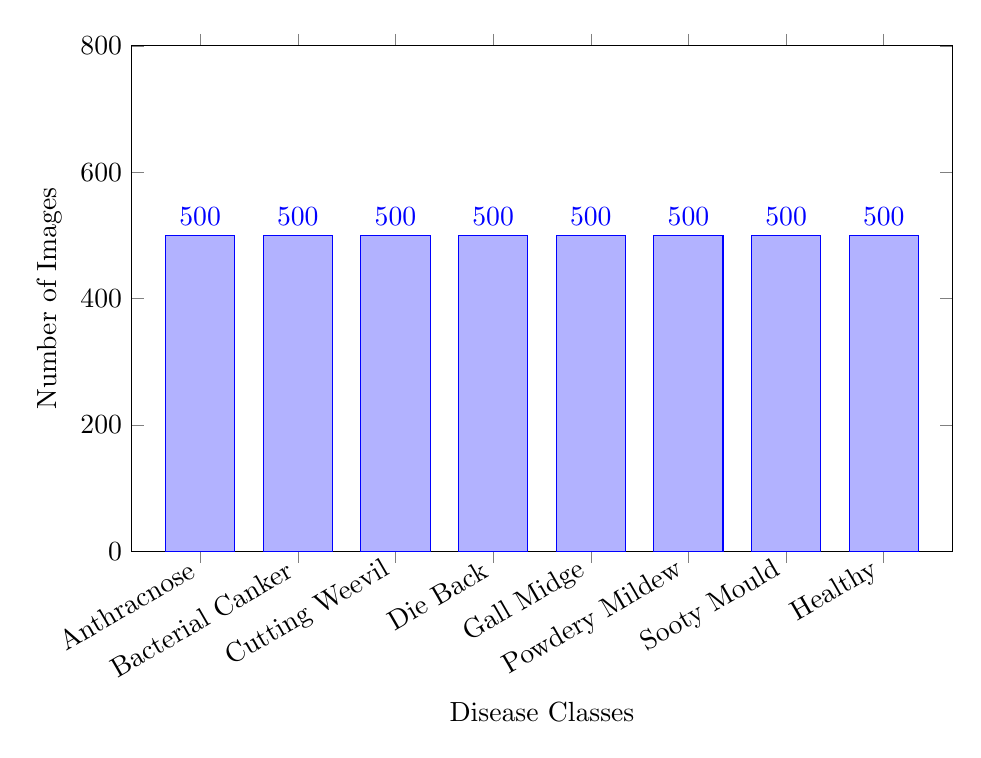
\begin{tikzpicture}
\begin{axis}[
    width=12cm,
    height=8cm,
    ybar,
    bar width=25pt,
    xlabel={Disease Classes},
    ylabel={Number of Images},
    symbolic x coords={Anthracnose,Bacterial Canker,Cutting Weevil,Die Back,Gall Midge,Powdery Mildew,Sooty Mould,Healthy},
    xtick=data,
    nodes near coords,
    enlarge x limits=0.1,
    xticklabel style={rotate=30, anchor=east},
    ymin=0, ymax= 800,
    ylabel near ticks,
    xlabel near ticks
]
\addplot coordinates {
    (Anthracnose,500)
    (Bacterial Canker,500)
    (Cutting Weevil,500)
    (Die Back,500)
    (Gall Midge,500)
    (Powdery Mildew,500)
    (Sooty Mould,500)
    (Healthy,500)
};
\end{axis}
\end{tikzpicture}
\end{figure}

\subsection{Disease Classes and Their Visual Features}

Each class in the dataset represents a specific mango leaf condition. Understanding the visual characteristics of each disease is important for both human inspection and model interpretability.

\begin{table}[H]
\centering
\caption{Visual Characteristics of Each Class}
\label{tab:disease-characteristics}
\renewcommand{\arraystretch}{1.5}
\begin{adjustbox}{width=\textwidth}
\begin{tabular}{@{}p{3.5cm}p{12cm}@{}}
\toprule
\textbf{Disease Class} & \textbf{Key Visual Characteristics} \\
\midrule
\textbf{Anthracnose} & Small, dark brown to black lesions with irregular shapes. Commonly starts at the leaf tip and may coalesce to form large necrotic areas. Lesions often have a concentric ring pattern and may lead to leaf curling or drying. \\

\textbf{Bacterial Canker} & Water-soaked lesions that enlarge and turn dark brown or black. Lesions are often angular and surrounded by yellow halos. Severe cases show cracking along veins and deformation of the leaf surface. \\

\textbf{Cutting Weevil} & Leaves show notched, chewed, or semi-circular cuts along the margins, caused by adult weevils feeding. Damage appears as clean cuts and may affect multiple edges of a single leaf. \\

\textbf{Die Back} & Yellowing and browning begins at the tip and progresses downward toward the base. May cause full leaf drying and extend into twigs. Often associated with poor plant vigor or fungal infection. \\

\textbf{Gall Midge} & Distinct swollen blisters, wart-like growths, or raised galls appear on leaf surfaces, particularly near veins. Caused by insect larvae feeding inside the tissue. \\

\textbf{Powdery Mildew} & A whitish or gray powder-like fungal coating appears on both surfaces, but mainly on the upper side. Advanced stages cover large areas and may distort leaves. \\

\textbf{Sooty Mould} & A black, soot-like fungal layer covers the leaf surface. Although the mold itself does not infect the plant, it blocks sunlight and photosynthesis. Often linked to honeydew secretions from insects. \\

\textbf{Healthy} & Uniform bright green color, smooth texture, no visible signs of necrosis, deformation, or discoloration. Veins and edges are clearly defined and free of lesions or foreign growth. \\
\bottomrule
\end{tabular}
\end{adjustbox}
\end{table}

\begin{figure}[h!]
    \centering
    \includegraphics[width=1.0\textwidth]{Figure/leaf.pdf}
    \caption{Representative Images of Each Class}
    \label{fig:pdf_example}
\end{figure}



These images and visual descriptions help in understanding the symptom patterns for each disease and serve as a visual reference for model training and evaluation.

\chapter{Methodology}
\section{Dataset Preparation}

This study used a publicly available Mango Leaf Disease Dataset from Kaggle, which contains 4,000 images of healthy and diseased mango leaves captured under natural lighting conditions with a uniform background. The dataset includes eight categories: Anthracnose, Bacterial Canker, Cutting Weevil, Die Back, Gall Midge, Powdery Mildew, Sooty Mould and Healthy.\\
All images were visually inspected for quality and resized to a uniform resolution of 224$\times$224 pixels to ensure compatibility across all convolutional neural network (CNN) models. The dataset was then divided into training, validation, and testing subsets using stratified sampling to maintain balanced class representation.

\subsection{Supervised Dataset Preparation}

In the supervised learning setup, all samples were treated as labeled. The dataset was divided into \textbf{80\% for training}, \textbf{10\% for validation}, and \textbf{10\% for testing}, resulting in 3,200, 400, and 400 images, respectively.  

\begin{figure}[H]
\centering
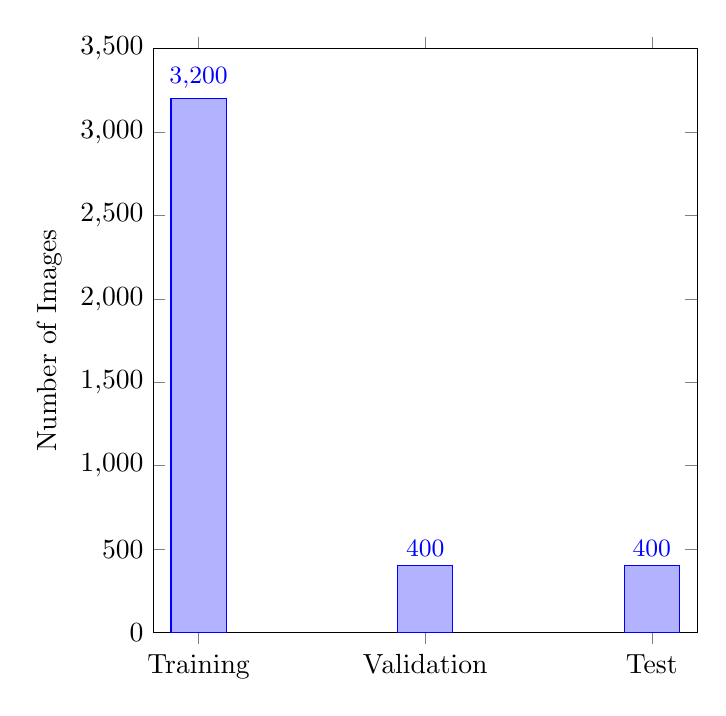
\begin{tikzpicture}
\begin{axis}[
    ybar,
    width=0.7\textwidth,
    height=9cm, % increased height
    bar width=20pt,
    ylabel={Number of Images},
    symbolic x coords={Training, Validation, Test},
    xtick=data,
    nodes near coords,
    every node near coord/.append style={font=\small},
    ymin=0,
    ymax=3500 % optional: make top of axis a bit higher than largest bar
]
\addplot coordinates {(Training,3200) (Validation,400) (Test,400)};
\end{axis}
\end{tikzpicture}
\caption{Supervised dataset split across training, validation, and test sets.}
\label{fig:supervised_split_simple}
\end{figure}
All images were normalized to pixel values between 0 and 1. The validation set was used for model tuning and early stopping, while the test set was used exclusively for the final evaluation. This preprocessing ensured the model was trained on a diverse yet balanced dataset, minimizing overfitting and improving robustness.

\subsection{Semi-Supervised Dataset Preparation}

For the semi-supervised setup, the same dataset was used, but with a reduced number of labeled samples to simulate limited annotation scenarios. From the total dataset, 80\% was used for training, 10\% for validation, and 10\% for testing. Within the training subset, only \textbf{25\% (800 images)} were labeled, while the remaining \textbf{75\% (2,400 images)} were treated as unlabeled. Class balance was maintained within the labeled portion.  

\begin{figure}[H]
\centering
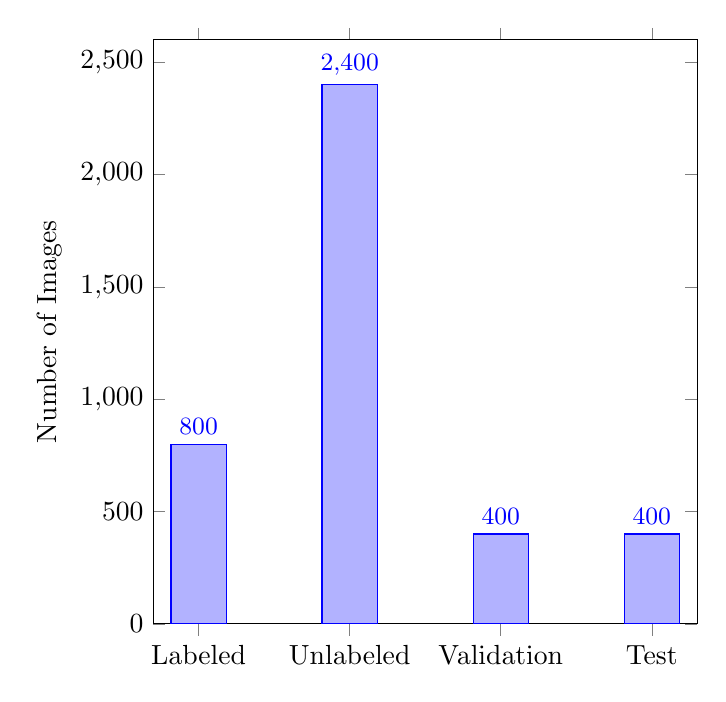
\begin{tikzpicture}
\begin{axis}[
    ybar,
    width=0.7\textwidth,
    height=9cm, % increased height
    bar width=20pt,
    ylabel={Number of Images},
    symbolic x coords={Labeled, Unlabeled, Validation, Test},
    xtick=data,
    nodes near coords,
    every node near coord/.append style={font=\small},
    ymin=0,
    ymax=2600 % slightly higher than the largest bar
]
\addplot coordinates {(Labeled,800) (Unlabeled,2400) (Validation,400) (Test,400)};
\end{axis}
\end{tikzpicture}
\caption{Semi-supervised dataset split showing labeled, unlabeled, validation, and test samples.}
\label{fig:semi_supervised_split_simple}
\end{figure}
The validation and test sets were kept completely separate and were not used during any training phase.


\section{VGG16 Model Architecture with Adapted Dense Layers}

\subsection{Initial Model Configuration}
The VGG16 model is initialized with ImageNet pre-trained weights while excluding the top classification layers. The base model receives input images of size $224 \times 224 \times 3$. To adapt VGG16 for our mango leaf disease classification task, we added custom dense layers on top of the frozen convolutional base:
\begin{itemize}
    \item Global Average Pooling 2D layer to reduce spatial dimensions.
    \item Dense layer with 256 neurons, ReLU activation, and L2 regularization ($0.016$).
    \item Batch Normalization layer for training stability.
    \item Dropout layer (0.5) to prevent overfitting.
    \item Dense layer with 128 neurons, ReLU activation, and L2 regularization ($0.016$).
    \item Dropout layer (0.3) for further regularization.
    \item Output Dense layer with softmax activation for multi-class classification.
\end{itemize}

\begin{figure}[htbp]
\centering
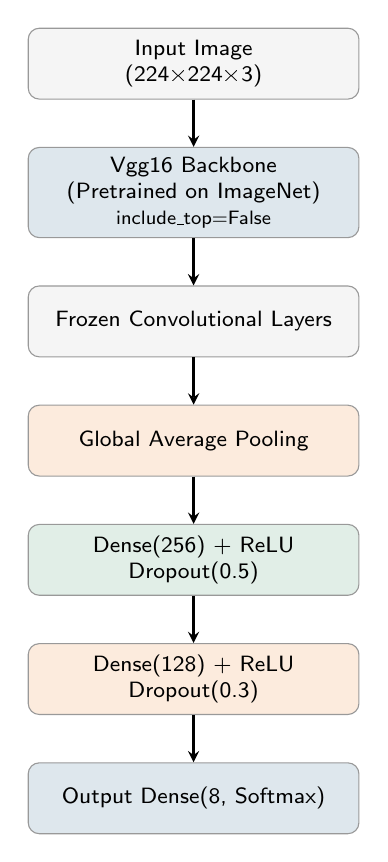
\begin{tikzpicture}[font=\sffamily\footnotesize, node distance=6mm,
layer/.style={rectangle, rounded corners=4pt, draw=black!40,
fill=#1!18, minimum width=4.2cm, minimum height=9mm, align=center},
arrow/.style={->, thick, >=stealth}
]

% Input
\node[layer=blockgray] (input) {Input Image\\(224×224×3)};

% ResNet101
\node[layer=blockblue, below=of input] (resnet)
{Vgg16 Backbone\\(Pretrained on ImageNet)\\\scriptsize include\_top=False};

% Freeze
\node[layer=blockgray, below=of resnet] (freeze)
{Frozen Convolutional Layers};

% GAP Layer
\node[layer=blockorange, below=of freeze] (gap)
{Global Average Pooling};

% Dense 1
\node[layer=blockgreen, below=of gap] (dense1)
{Dense(256) + ReLU\\Dropout(0.5)};

% Dense 2
\node[layer=blockorange, below=of dense1] (dense2)
{Dense(128) + ReLU\\Dropout(0.3)};

% Output
\node[layer=blockblue, below=of dense2] (output)
{Output Dense(8, Softmax)};

% Arrows
\draw[arrow] (input) -- (resnet);
\draw[arrow] (resnet) -- (freeze);
\draw[arrow] (freeze) -- (gap);
\draw[arrow] (gap) -- (dense1);
\draw[arrow] (dense1) -- (dense2);
\draw[arrow] (dense2) -- (output);

\end{tikzpicture}

\caption{Transfer learning model using Vgg16 as the feature extractor.}
\label{fig:resnet101_transfer_learning}
\end{figure}

\subsection{Supervised Training Strategy}
The supervised training was performed using a pre-trained VGG16 backbone with custom dense layers for classification. Let the input images be denoted as $\mathbf{X} \in \mathbb{R}^{H \times W \times C}$, where $H$ and $W$ are the height and width, and $C$ is the number of channels. The target labels are one-hot encoded vectors $\mathbf{Y} \in \{0,1\}^{n_\text{classes}}$. The model outputs predictions $\hat{\mathbf{Y}}$ through the softmax function \cite{wang2018high}:

\[
\hat{y}_i = \frac{e^{z_i}}{\sum_{j=1}^{n_\text{classes}} e^{z_j}}, \quad i = 1,2,\dots,n_\text{classes},
\]
where $z_i$ are the logits from the final dense layer. The training minimizes the \textbf{categorical cross-entropy loss} \cite{zhang2018generalized}:

\[
\mathcal{L}(\mathbf{Y}, \hat{\mathbf{Y}}) = - \sum_{i=1}^{n_\text{classes}} y_i \log(\hat{y}_i).
\]
Initially, the VGG16 base was \textbf{frozen}, and only the added dense layers were trained using the \textbf{Adamax optimizer} with learning rate $\eta = 10^{-3}$. Early stopping with a patience of 10 epochs and model checkpointing were employed to prevent overfitting. To improve generalization, \textbf{dropout} layers and L2 regularization ($\lambda \|\mathbf{W}\|_2^2$) were applied in the dense layers, where $\mathbf{W}$ denotes the layer weights. The training process was monitored using the accuracy metric:
\[
\text{Accuracy} = \frac{\text{Number of correct predictions}}{\text{Total number of predictions}}.
\]
Finally, the model was evaluated on the validation and test sets, and training progress was visualized through plots of loss $\mathcal{L}$ and accuracy across epochs.

\subsection{Semi-supervised Fine-Tuning the Model}
The semi-supervised approach enhances the model by leveraging unlabeled data:
\begin{itemize}
    \item \textbf{Phase 1:} Initial training on only 25\% of the labeled training data, following the same  approach as supervised learning.
    \item \textbf{Pseudo-labeling:} The model trained on limited labeled data is used to generate predictions on the remaining unlabeled data. Samples with prediction confidence above 95\% are added to the training set with their predicted labels.
    \item \textbf{Phase 2:} The model is fine-tuned on the combined dataset (original labeled data + high-confidence pseudo-labeled data). The top 4 layers of VGG16 are unfrozen, and the model is trained with a very low learning rate ($10^{-5}$) for up to 100 epochs with early stopping and learning rate reduction \cite{hady2013semi}.
\end{itemize}

\section{MobileNetV2 Model Architecture with Adapted Dense Layers}

\subsubsection{Initial Model Configuration}
MobileNetV2 is initialized with ImageNet pre-trained weights without its top classification layers. The model accepts $224 \times 224 \times 3$ input images. For our specific task, we added custom dense layers:
\begin{itemize}
    \item Global Average Pooling 2D layer.
    \item Dense layer with 256 neurons, ReLU activation, and L2 regularization ($0.016$).
    \item Batch Normalization layer.
    \item Dropout layer (0.5).
    \item Dense layer with 128 neurons, ReLU activation, and L2 regularization ($0.016$).
    \item Dropout layer (0.3).
    \item Output Dense layer with softmax activation.
\end{itemize}

\begin{figure}[htbp]
\centering
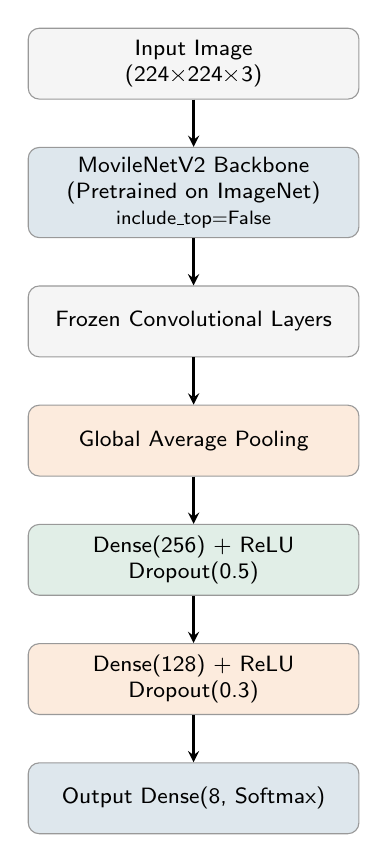
\begin{tikzpicture}[font=\sffamily\footnotesize, node distance=6mm,
layer/.style={rectangle, rounded corners=4pt, draw=black!40,
fill=#1!18, minimum width=4.2cm, minimum height=9mm, align=center},
arrow/.style={->, thick, >=stealth}
]

% Input
\node[layer=blockgray] (input) {Input Image\\(224×224×3)};

% ResNet101
\node[layer=blockblue, below=of input] (resnet)
{MovileNetV2 Backbone\\(Pretrained on ImageNet)\\\scriptsize include\_top=False};

% Freeze
\node[layer=blockgray, below=of resnet] (freeze)
{Frozen Convolutional Layers};

% GAP Layer
\node[layer=blockorange, below=of freeze] (gap)
{Global Average Pooling};

% Dense 1
\node[layer=blockgreen, below=of gap] (dense1)
{Dense(256) + ReLU\\Dropout(0.5)};

% Dense 2
\node[layer=blockorange, below=of dense1] (dense2)
{Dense(128) + ReLU\\Dropout(0.3)};

% Output
\node[layer=blockblue, below=of dense2] (output)
{Output Dense(8, Softmax)};

% Arrows
\draw[arrow] (input) -- (resnet);
\draw[arrow] (resnet) -- (freeze);
\draw[arrow] (freeze) -- (gap);
\draw[arrow] (gap) -- (dense1);
\draw[arrow] (dense1) -- (dense2);
\draw[arrow] (dense2) -- (output);

\end{tikzpicture}

\caption{Transfer learning model using MobileNetV2 as the feature extractor.}
\label{fig:resnet101_transfer_learning}
\end{figure}


\subsection{Supervised Training Strategy}
The supervised training was performed using a pre-trained MobileNetV2 backbone with custom dense layers for classification. Let the input images be denoted as $\mathbf{X} \in \mathbb{R}^{H \times W \times C}$, where $H$ and $W$ are the height and width, and $C$ is the number of channels. The target labels are one-hot encoded vectors $\mathbf{Y} \in \{0,1\}^{n_\text{classes}}$. The model outputs predictions $\hat{\mathbf{Y}}$ through the softmax function:

\[
\hat{y}_i = \frac{e^{z_i}}{\sum_{j=1}^{n_\text{classes}} e^{z_j}}, \quad i = 1,2,\dots,n_\text{classes},
\]
where $z_i$ are the logits from the final dense layer. The training minimizes the \textbf{categorical cross-entropy loss}:

\[
\mathcal{L}(\mathbf{Y}, \hat{\mathbf{Y}}) = - \sum_{i=1}^{n_\text{classes}} y_i \log(\hat{y}_i).
\]
Initially, the MobileNetV2 base was \textbf{frozen}, and only the added dense layers were trained using the \textbf{Adamax optimizer} with learning rate $\eta = 10^{-3}$. Early stopping with a patience of 10 epochs and model checkpointing were employed to prevent overfitting. To improve generalization, \textbf{dropout} layers and L2 regularization ($\lambda \|\mathbf{W}\|_2^2$) were applied in the dense layers, where $\mathbf{W}$ denotes the layer weights. The training process was monitored using the accuracy metric:
\[
\text{Accuracy} = \frac{\text{Number of correct predictions}}{\text{Total number of predictions}}.
\]
Finally, the model was evaluated on the validation and test sets, and training progress was visualized through plots of loss $\mathcal{L}$ and accuracy across epochs.

\subsection{Semi-supervised Fine-Tuning the Model}
The semi-supervised approach for MobileNetV2 follows the same pattern as VGG16:
\begin{itemize}
    \item \textbf{Phase 1:} Initial training on only 25\% of the labeled data with the two-stage approach.
    \item \textbf{Pseudo-labeling:} The model generates predictions on unlabeled data, with high-confidence samples ($\geq$95\%) added to the training set.
    \item \textbf{Phase 2:} Fine-tuning on the combined dataset with the top 20 layers of MobileNetV2 unfrozen, using a very low learning rate ($10^{-5}$) for up to 100 epochs with early stopping and learning rate reduction \cite{hady2013semi}.
\end{itemize}

\section{ResNet101 Model Architecture with Adapted Dense Layers}

\subsection{Initial Model Configuration}
ResNet101 is initialized with ImageNet pre-trained weights, excluding the top classification layers. The model processes $224 \times 224 \times 3$ input images. The custom dense layers added for our task include:
\begin{itemize}
    \item Global Average Pooling 2D layer.
    \item Dense layer with 256 neurons, ReLU activation, and L2 regularization ($0.016$).
    \item Batch Normalization layer.
    \item Dropout layer (0.5).
    \item Dense layer with 128 neurons, ReLU activation, and L2 regularization ($0.016$).
    \item Dropout layer (0.3).
    \item Output Dense layer with softmax activation.
\end{itemize}
\begin{figure}[htbp]
\centering
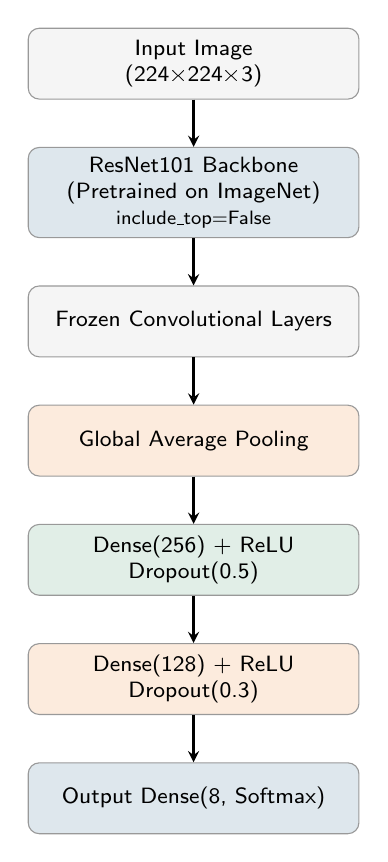
\begin{tikzpicture}[font=\sffamily\footnotesize, node distance=6mm,
layer/.style={rectangle, rounded corners=4pt, draw=black!40,
fill=#1!18, minimum width=4.2cm, minimum height=9mm, align=center},
arrow/.style={->, thick, >=stealth}
]

% Input
\node[layer=blockgray] (input) {Input Image\\(224×224×3)};

% ResNet101
\node[layer=blockblue, below=of input] (resnet)
{ResNet101 Backbone\\(Pretrained on ImageNet)\\\scriptsize include\_top=False};

% Freeze
\node[layer=blockgray, below=of resnet] (freeze)
{Frozen Convolutional Layers};

% GAP Layer
\node[layer=blockorange, below=of freeze] (gap)
{Global Average Pooling};

% Dense 1
\node[layer=blockgreen, below=of gap] (dense1)
{Dense(256) + ReLU\\Dropout(0.5)};

% Dense 2
\node[layer=blockorange, below=of dense1] (dense2)
{Dense(128) + ReLU\\Dropout(0.3)};

% Output
\node[layer=blockblue, below=of dense2] (output)
{Output Dense(8, Softmax)};

% Arrows
\draw[arrow] (input) -- (resnet);
\draw[arrow] (resnet) -- (freeze);
\draw[arrow] (freeze) -- (gap);
\draw[arrow] (gap) -- (dense1);
\draw[arrow] (dense1) -- (dense2);
\draw[arrow] (dense2) -- (output);

\end{tikzpicture}

\caption{Transfer learning model using ResNet101 as the feature extractor.}
\label{fig:resnet101_transfer_learning}
\end{figure}


\subsection{Supervised Training Strategy}
The supervised training was performed using a pre-trained ResNet101 backbone with custom dense layers for classification. Let the input images be denoted as $\mathbf{X} \in \mathbb{R}^{H \times W \times C}$, where $H$ and $W$ are the height and width, and $C$ is the number of channels. The target labels are one-hot encoded vectors $\mathbf{Y} \in \{0,1\}^{n_\text{classes}}$. The model outputs predictions $\hat{\mathbf{Y}}$ through the softmax function:

\[
\hat{y}_i = \frac{e^{z_i}}{\sum_{j=1}^{n_\text{classes}} e^{z_j}}, \quad i = 1,2,\dots,n_\text{classes},
\]
where $z_i$ are the logits from the final dense layer. The training minimizes the \textbf{categorical cross-entropy loss}:

\[
\mathcal{L}(\mathbf{Y}, \hat{\mathbf{Y}}) = - \sum_{i=1}^{n_\text{classes}} y_i \log(\hat{y}_i).
\]
Initially, the ResNet101 base was \textbf{frozen}, and only the added dense layers were trained using the \textbf{Adamax optimizer} with learning rate $\eta = 10^{-3}$. Early stopping with a patience of 10 epochs and model checkpointing were employed to prevent overfitting. To improve generalization, \textbf{dropout} layers and L2 regularization ($\lambda \|\mathbf{W}\|_2^2$) were applied in the dense layers, where $\mathbf{W}$ denotes the layer weights. The training process was monitored using the accuracy metric:
\[
\text{Accuracy} = \frac{\text{Number of correct predictions}}{\text{Total number of predictions}}.
\]
Finally, the model was evaluated on the validation and test sets, and training progress was visualized through plots of loss $\mathcal{L}$ and accuracy across epochs.
\subsection{Semi-supervised Fine-Tuning the Model}
The semi-supervised approach for ResNet101 follows the same pattern:
\begin{itemize}
    \item \textbf{Phase 1:} Initial training on only 25\% of the labeled data with the two-stage approach.
    \item \textbf{Pseudo-labeling:} The model generates predictions on unlabeled data, with high-confidence samples ($\geq$95\%) added to the training set.
    \item \textbf{Phase 2:} Fine-tuning on the combined dataset with the top 30 layers of ResNet101 unfrozen, using a very low learning rate ($10^{-5}$) for up to 100 epochs with early stopping and learning rate reduction \cite{hady2013semi}.
\end{itemize}

\section{DenseNet121 Model Architecture with Adapted Dense Layers}

\subsection{Initial Model Configuration}
DenseNet121 is initialized with ImageNet pre-trained weights, excluding the top classification layers. The model accepts $224 \times 224 \times 3$ input images. The custom dense layers added for our task include:
\begin{itemize}
    \item Global Average Pooling 2D layer.
    \item Dense layer with 256 neurons, ReLU activation, and L2 regularization ($0.016$).
    \item Batch Normalization layer.
    \item Dropout layer (0.5).
    \item Dense layer with 128 neurons, ReLU activation, and L2 regularization ($0.016$).
    \item Dropout layer (0.3).
    \item Output Dense layer with softmax activation.
\end{itemize}

\begin{figure}[htbp]
\centering
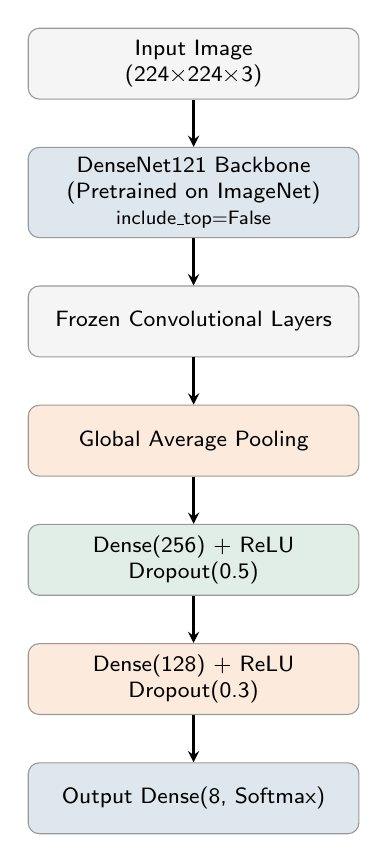
\begin{tikzpicture}[font=\sffamily\footnotesize, node distance=6mm,
layer/.style={rectangle, rounded corners=4pt, draw=black!40,
fill=#1!18, minimum width=4.2cm, minimum height=9mm, align=center},
arrow/.style={->, thick, >=stealth}
]

% Input
\node[layer=blockgray] (input) {Input Image\\(224×224×3)};

% ResNet101
\node[layer=blockblue, below=of input] (resnet)
{DenseNet121 Backbone\\(Pretrained on ImageNet)\\\scriptsize include\_top=False};

% Freeze
\node[layer=blockgray, below=of resnet] (freeze)
{Frozen Convolutional Layers};

% GAP Layer
\node[layer=blockorange, below=of freeze] (gap)
{Global Average Pooling};

% Dense 1
\node[layer=blockgreen, below=of gap] (dense1)
{Dense(256) + ReLU\\Dropout(0.5)};

% Dense 2
\node[layer=blockorange, below=of dense1] (dense2)
{Dense(128) + ReLU\\Dropout(0.3)};

% Output
\node[layer=blockblue, below=of dense2] (output)
{Output Dense(8, Softmax)};

% Arrows
\draw[arrow] (input) -- (resnet);
\draw[arrow] (resnet) -- (freeze);
\draw[arrow] (freeze) -- (gap);
\draw[arrow] (gap) -- (dense1);
\draw[arrow] (dense1) -- (dense2);
\draw[arrow] (dense2) -- (output);

\end{tikzpicture}

\caption{Transfer learning model using DenseNet121 as the feature extractor.}
\label{fig:resnet101_transfer_learning}
\end{figure}



\subsection{Supervised Training Strategy}
The supervised training was performed using a pre-trained DenseNet121 backbone with custom dense layers for classification. Let the input images be denoted as $\mathbf{X} \in \mathbb{R}^{H \times W \times C}$, where $H$ and $W$ are the height and width, and $C$ is the number of channels. The target labels are one-hot encoded vectors $\mathbf{Y} \in \{0,1\}^{n_\text{classes}}$. The model outputs predictions $\hat{\mathbf{Y}}$ through the softmax function \cite{wang2018high}:

\[
\hat{y}_i = \frac{e^{z_i}}{\sum_{j=1}^{n_\text{classes}} e^{z_j}}, \quad i = 1,2,\dots,n_\text{classes},
\]
where $z_i$ are the logits from the final dense layer. The training minimizes the \textbf{categorical cross-entropy loss}:

\[
\mathcal{L}(\mathbf{Y}, \hat{\mathbf{Y}}) = - \sum_{i=1}^{n_\text{classes}} y_i \log(\hat{y}_i).
\]
Initially, the DenseNet121 base was \textbf{frozen}, and only the added dense layers were trained using the \textbf{Adamax optimizer} with learning rate $\eta = 10^{-3}$. Early stopping with a patience of 10 epochs and model checkpointing were employed to prevent overfitting. To improve generalization, \textbf{dropout} layers and L2 regularization ($\lambda \|\mathbf{W}\|_2^2$) were applied in the dense layers, where $\mathbf{W}$ denotes the layer weights. The training process was monitored using the accuracy metric:
\[
\text{Accuracy} = \frac{\text{Number of correct predictions}}{\text{Total number of predictions}}.
\]
Finally, the model was evaluated on the validation and test sets, and training progress was visualized through plots of loss $\mathcal{L}$ and accuracy across epochs.
\subsection{Semi-supervised Fine-Tuning the Model}
The semi-supervised approach for DenseNet121 follows the same pattern:
\begin{itemize}
    \item \textbf{Phase 1:} Initial training on only 25\% of the labeled data with the two-stage approach.
    \item \textbf{Pseudo-labeling:} The model generates predictions on unlabeled data, with high-confidence samples ($\geq$95\%) added to the training set.
    \item \textbf{Phase 2:} Fine-tuning on the combined dataset with the top 15 layers of DenseNet121 unfrozen, using a very low learning rate ($10^{-5}$) for up to 100 epochs with early stopping and learning rate reduction \cite{hady2013semi}.
\end{itemize}

\section{Proposed Model Architecture for Supervised and Semi-supervised Classification}

\subsection{Overall Architecture Design}

The proposed model is a custom Convolutional Neural Network (CNN) comprising four convolutional blocks followed by a classification head. Unlike the pre-trained models (VGG16, ResNet101, MobileNetV2, and DenseNet121) that were originally designed for ImageNet classification, this architecture is specifically tailored for the characteristics of mango leaf disease images, providing a balance between model complexity and computational efficiency while preventing overfitting on limited labeled data.\\
The architecture accepts input images of size 224×224×3 pixels and outputs probability distributions across eight disease classes. The model contains approximately 3.5 million trainable parameters, making it significantly more lightweight than the baseline models while maintaining competitive performance.
\begin{figure}[htbp!]
\centering
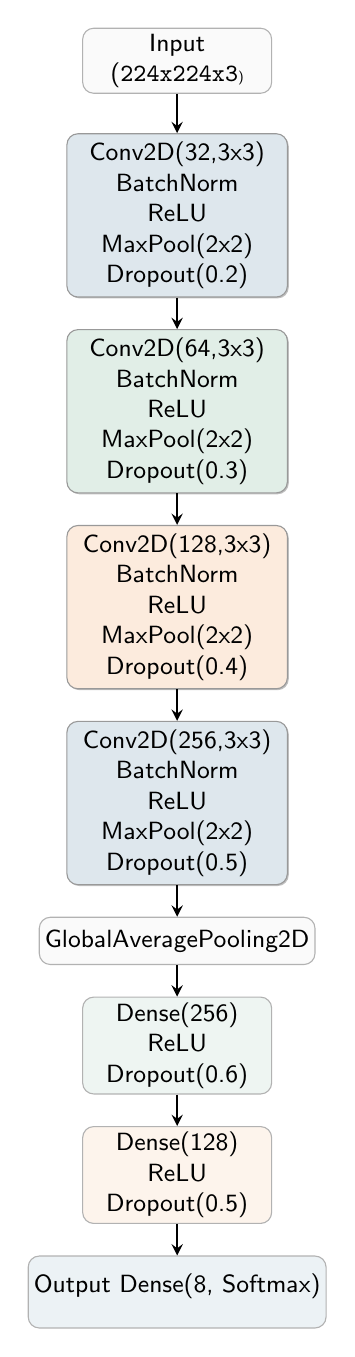
\begin{tikzpicture}[font=\sffamily\small
, every node/.style={align=center},
    layer/.style={rectangle, rounded corners=4pt, draw=black!40, fill=#1!18, minimum width=2.8cm, minimum height=7mm, inner sep=3pt, drop shadow={shadow xshift=0.5pt, shadow yshift=-0.5pt}},
    smalllayer/.style={rectangle, rounded corners=4pt, draw=black!30, fill=#1!10, minimum width=2.4cm, minimum height=6mm, inner sep=2pt},
    arrow/.style={->, thick, rounded corners=2pt, >=stealth}
]

% Input
\node (input) [smalllayer={blockgray}] {Input\\(\tiny \texttt{\small 224x224x3})};

% Block 1
\node (b1) [layer={blockblue}, below=5mm of input] {Conv2D(32,3x3)\\BatchNorm\\ReLU\\MaxPool(2x2)\\Dropout(0.2)};

% Block 2
\node (b2) [layer={blockgreen}, below=4mm of b1] {Conv2D(64,3x3)\\BatchNorm\\ReLU\\MaxPool(2x2)\\Dropout(0.3)};

% Block 3
\node (b3) [layer={blockorange}, below=4mm of b2] {Conv2D(128,3x3)\\BatchNorm\\ReLU\\MaxPool(2x2)\\Dropout(0.4)};

% Block 4
\node (b4) [layer={blockblue}, below=4mm of b3] {Conv2D(256,3x3)\\BatchNorm\\ReLU\\MaxPool(2x2)\\Dropout(0.5)};

% Global Pooling & Head
\node (gap) [smalllayer={blockgray}, below=4mm of b4] {GlobalAveragePooling2D};
\node (d1) [smalllayer={blockgreen}, below=4mm of gap] {Dense(256)\\ReLU\\Dropout(0.6)};
\node (d2) [smalllayer={blockorange}, below=4mm of d1] {Dense(128)\\ReLU\\Dropout(0.5)};
\node (out) [smalllayer={blockblue}, below=4mm of d2] {\\Output Dense(8, Softmax)\\};

% Connections
\draw[arrow] (input) -- (b1);
\draw[arrow] (b1) -- (b2);
\draw[arrow] (b2) -- (b3);
\draw[arrow] (b3) -- (b4);
\draw[arrow] (b4) -- (gap);
\draw[arrow] (gap) -- (d1);
\draw[arrow] (d1) -- (d2);
\draw[arrow] (d2) -- (out);

\end{tikzpicture}
\caption{Proposed CNN architecture for mango leaf disease classification.}
\label{fig:cnn_architecture}
\end{figure}

\subsection{Convolutional Block Design}

The proposed architecture consists of four hierarchical convolutional blocks, each following a consistent design pattern. The mathematical formulation of the core convolution operation is:

\subsubsection*{Convolutional Operation:}

The convolution operation at layer $l$ is defined as:

\begin{equation}
z^{[l]} = W^{[l]} * a^{[l-1]} + b^{[l]}
\end{equation}

where $W^{[l]}$ represents the learnable filters, $*$ denotes the convolution operation, $a^{[l-1]}$ is the input activation from the previous layer, and $b^{[l]}$ is the bias term.

\subsubsection*{Block 1 (Input Processing):}
\begin{itemize}
    \item Conv2D layer: 32 filters, 3×3 kernel, same padding, L2 regularization (1e-4)
    \item Batch Normalization layer
    \item ReLU activation
    \item Max Pooling: 2×2 pool size
    \item Dropout: 20\% rate
\end{itemize}

\subsubsection*{Block 2 (Feature Extraction):}
\begin{itemize}
    \item Conv2D layer: 64 filters, 3×3 kernel, same padding, L2 regularization (1e-4)
    \item Batch Normalization layer
    \item ReLU activation
    \item Max Pooling: 2×2 pool size
    \item Dropout: 30\% rate
\end{itemize}

\subsubsection*{Block 3 (Mid-level Features):}
\begin{itemize}
    \item Conv2D layer: 128 filters, 3×3 kernel, same padding, L2 regularization (1e-4)
    \item Batch Normalization layer
    \item ReLU activation
    \item Max Pooling: 2×2 pool size
    \item Dropout: 40\% rate
\end{itemize}

\subsubsection*{Block 4 (High-level Features):}
\begin{itemize}
    \item Conv2D layer: 256 filters, 3×3 kernel, same padding, L2 regularization (1e-4)
    \item Batch Normalization layer
    \item ReLU activation
    \item Max Pooling: 2×2 pool size
    \item Dropout: 50\% rate
\end{itemize}
Each block progressively increases both the number of filters (32→64→128→256) and the dropout rate (0.2→0.3→0.4→0.5), enabling the network to learn increasingly complex features while maintaining strong regularization to prevent overfitting.

\subsection{Activation and Pooling Operations}

\subsubsection{ReLU Activation Function}

The Rectified Linear Unit (ReLU) activation function is applied after batch normalization in each convolutional block \cite{schmidt2020nonparametric}:

\begin{equation}
\text{ReLU}(x) = \max(0, x) = \begin{cases} 
x & \text{if } x > 0 \\
0 & \text{if } x \leq 0
\end{cases}
\end{equation}
ReLU introduces non-linearity while maintaining computational efficiency and mitigating the vanishing gradient problem.

\subsubsection{Max Pooling Operation}

Max pooling with 2×2 window reduces spatial dimensions by selecting the maximum value in each pooling region:

\begin{equation}
y_{i,j} = \max_{(p,q) \in \mathcal{R}_{i,j}} x_{p,q}
\end{equation}
where $\mathcal{R}_{i,j}$ represents the 2×2 pooling region corresponding to output position $(i,j)$.

\subsubsection{Dropout Regularization}

During training, dropout randomly sets a fraction $p$ of neurons to zero:

\begin{equation}
\tilde{a}^{[l]} = a^{[l]} \odot m
\end{equation}

where $m \sim \text{Bernoulli}(1-p)$ is a binary mask, and $\odot$ denotes element-wise multiplication. During inference, activations are scaled by $(1-p)$ to maintain expected values.

\subsection{Classification Head}

Following the convolutional blocks, the classification head processes the extracted features through global average pooling and fully connected layers.

\subsubsection{Global Average Pooling}

For feature maps of spatial dimensions $H \times W$ with $C$ channels, global average pooling computes:

\begin{equation}
\text{GAP}_c = \frac{1}{H \times W}\sum_{i=1}^{H}\sum_{j=1}^{W}x_{i,j,c}
\end{equation}

This reduces each feature map to a single value, resulting in a $C$-dimensional vector (256 dimensions from the final convolutional block).

\subsubsection*{Fully Connected Layers:}
\begin{itemize}
    \item Dense Layer 1: 256 units with ReLU activation and L2 regularization (1e-4)
    \item Dropout: 60\% rate
    \item Dense Layer 2: 128 units with ReLU activation and L2 regularization (1e-4)
    \item Dropout: 50\% rate
    \item Output Layer: 8 units with softmax activation
\end{itemize}

\subsubsection{Softmax Activation Function}

The output layer uses softmax activation to produce probability distributions over the 8 disease classes:

\begin{equation}
\text{softmax}(z_i) = \frac{e^{z_i}}{\sum_{j=1}^{K}e^{z_j}}
\end{equation}

where $K=8$ is the number of disease classes, $z_i$ is the logit for class $i$, and the output represents $P(y=i|x)$, the probability of input $x$ belonging to class $i$.

\subsection{Regularization Strategy}

To address the challenge of overfitting on small datasets, the proposed model incorporates multiple regularization techniques:

\subsubsection{L2 Weight Regularization}

All convolutional and dense layers employ L2 regularization with coefficient 1e-4, which adds a penalty term to the loss function that penalizes large weights and promotes model generalization.

\subsubsection{Progressive Dropout}

Dropout rates increase progressively through the network (20\%→30\%→40\%→50\%→60\%→50\%), with the highest rates applied to the fully connected layers where overfitting is most likely to occur. This stochastic regularization technique forces the network to learn robust features that are not dependent on specific neuron activations.

\subsubsection{Batch Normalization}

Applied after each convolutional layer to normalize activations, stabilize training, and provide mild regularization effects. Batch normalization reduces internal covariate shift and allows for higher learning rates during training.

\subsection{Data Augmentation Strategies}

The model employs aggressive data augmentation techniques specifically designed for leaf disease images to artificially expand the training dataset and improve model generalization.

\subsubsection*{Training Augmentation:}
\begin{itemize}
    \item Rotation: Random rotations up to ±40°
    \item Translation: Horizontal and vertical shifts up to 25\%
    \item Shear transformation: Intensity of 0.2
    \item Zoom: Random zoom in/out up to 25\%
    \item Horizontal flip: Random horizontal flipping (50\% probability)
    \item Vertical flip: Random vertical flipping (50\% probability) - as leaves can appear in any orientation
    \item Brightness adjustment: Random brightness variation between 0.7× and 1.3×
    \item Channel shift: RGB channel intensity shifts up to ±20
    \item Normalization: Pixel values rescaled to [0, 1]
\end{itemize}

\subsubsection*{Validation/Test Augmentation:}
\begin{itemize}
    \item Only pixel normalization (rescaling to [0, 1]) is applied to ensure consistent evaluation.
\end{itemize}

\subsection{Supervised Learning Framework}

The supervised learning approach utilizes all available labeled data for training with careful data splitting and class balancing strategies.

\subsubsection{Data Splitting Strategy}

\begin{itemize}
    \item Training set: 80\% of total data
    \item Validation set: 10\% of total data
    \item Test set: 10\% of total data
\end{itemize}
All splits maintain class stratification to ensure balanced representation across disease categories, preventing bias toward dominant classes during training and evaluation.

\subsubsection{Loss Function}

The model is trained using categorical cross-entropy loss with class weighting to handle imbalanced datasets:

\begin{equation}
\mathcal{L}_{\text{CE}} = -\frac{1}{N}\sum_{i=1}^{N}w_{y_i}\sum_{c=1}^{K}y_{i,c}\log(\hat{y}_{i,c})
\end{equation}

where:
\begin{itemize}
    \item $N$ is the number of samples in the batch
    \item $K=8$ is the number of classes
    \item $y_{i,c}$ is the ground truth (1 if sample $i$ belongs to class $c$, 0 otherwise)
    \item $\hat{y}_{i,c}$ is the predicted probability for class $c$
    \item $w_{y_i}$ is the class weight for the true class of sample $i$
\end{itemize}
Class weights are computed using the balanced weighting scheme from scikit-learn, which assigns higher weights to minority classes to ensure fair representation during training.

\subsubsection{Optimization Algorithm}
The Adam (Adaptive Moment Estimation) optimizer is employed with the following configuration:
\begin{itemize}
    \item Initial learning rate: 1×10$^{-3}$
    \item Beta parameters: $\beta_1$=0.9, $\beta_2$=0.999 (default Adam parameters)
    \item Epsilon: 1×10$^{-7}$ for numerical stability
\end{itemize}

Adam combines the advantages of adaptive learning rates and momentum, making it well-suited for training deep neural networks with sparse gradients.

\subsubsection{Adaptive Learning Rate Strategy}

ReduceLROnPlateau callback adjusts the learning rate dynamically when validation accuracy plateaus:
\begin{itemize}
    \item Monitoring metric: Validation accuracy
    \item Reduction factor: 0.5 (halves the learning rate)
    \item Patience: 8 epochs without improvement
    \item Minimum learning rate: 1×10$^{-7}$
\end{itemize}

This adaptive strategy prevents overshooting optimal weights while allowing the model to escape shallow local minima.

\subsubsection{Training Configuration}

\begin{itemize}
    \item Batch Size: 32 samples
    \item Maximum Epochs: 100
    \item Early Stopping: Monitors validation accuracy with patience of 20 epochs, restoring best weights to prevent overfitting
\end{itemize}

\subsection{Semi-Supervised Learning Framework}

The semi-supervised approach extends the supervised model by leveraging unlabeled data through an iterative pseudo-labeling strategy, which is particularly beneficial when labeled data is scarce or expensive to obtain.

\subsubsection{Data Partitioning}

From the training set:
\begin{itemize}
    \item Labeled data: 25\% (with ground truth labels)
    \item Unlabeled data: 75\% (labels withheld for pseudo-labeling)
    \item Validation set: 10\% of original data (held out from both labeled and unlabeled pools)
    \item Test set: 10\% of original data (held out for final evaluation)
\end{itemize}
This partitioning simulates realistic scenarios where only a small fraction of data is labeled while abundant unlabeled data is available.

\subsubsection{Phase 1: Initial Supervised Training}

The model is first trained exclusively on the labeled subset (25\% of training data) to establish a baseline model capable of generating reliable pseudo-labels:

\begin{itemize}
    \item Training epochs: Up to 50 with early stopping (patience = 15 epochs)
    \item Initial learning rate: 5×10$^{-4}$ (lower than supervised to prevent overfitting on small labeled set)
    \item Learning rate reduction patience: 7 epochs
    \item Same loss function, optimizer, and regularization as supervised learning
\end{itemize}

This phase establishes a teacher model that demonstrates sufficient generalization capability on the validation set before proceeding to pseudo-labeling.

\subsubsection{Phase 2: Iterative Pseudo-Labeling}

The semi-supervised framework employs an iterative self-training approach with confidence-based selection and progressive threshold adjustment.

\subsubsection*{Configuration:}
\begin{itemize}
    \item Number of iterations: 4
    \item Initial confidence threshold: 0.70 (conservative start)
    \item Final confidence threshold: 0.90 (high-quality pseudo-labels)
    \item Minimum samples per iteration: 50
    \item Maximum samples per iteration: 300
\end{itemize}

\subsubsection*{Progressive Confidence Threshold:}

The confidence threshold increases linearly across iterations from 0.70 to 0.90, ensuring that:
\begin{itemize}
    \item Early iterations incorporate moderately confident predictions to expand the training set
    \item Later iterations focus only on highly confident predictions to maintain label quality
    \item Gradual progression prevents sudden distribution shifts in the training data
\end{itemize}

\subsubsection*{Test-Time Augmentation (TTA):}

To improve pseudo-label reliability, predictions for each unlabeled sample are averaged across 3 augmented versions of the image. This ensemble approach reduces prediction variance and increases confidence in selected samples by accounting for augmentation-induced variations.

\subsubsection*{Sample Selection Process:}

For each iteration:
\begin{enumerate}
    \item Model generates predictions on all remaining unlabeled samples using TTA
    \item Samples with maximum class probability exceeding the current threshold are selected
    \item If more than 300 samples qualify, only the top 300 most confident samples are chosen
    \item If fewer than 50 samples qualify, the iteration is skipped to prevent training instability
    \item Selected samples and their pseudo-labels are added to the training set
    \item These samples are removed from the unlabeled pool
\end{enumerate}

\subsubsection*{Pseudo-Label Distribution Analysis:}

At each iteration, the class distribution of pseudo-labels is analyzed and reported to ensure:
\begin{itemize}
    \item Balanced incorporation across disease classes
    \item No systematic bias toward dominant classes
    \item Detection of potential model biases that may propagate through iterations
\end{itemize}

\subsubsection{Iterative Fine-tuning Strategy}

After pseudo-label generation at each iteration, the model is retrained on the combined dataset (original labeled data + accumulated pseudo-labeled data):

\subsubsection*{Fine-tuning Configuration:}
\begin{itemize}
    \item Epochs per iteration: 20
    \item Early stopping patience: 8 epochs
    \item Learning rate reduction patience: 4 epochs
\end{itemize}

\subsubsection*{Adaptive Learning Rate Decay:}

The learning rate decreases by a factor of 1.5 at each iteration:
\begin{itemize}
    \item Iteration 1: 1.00×10$^{-4}$
    \item Iteration 2: 6.67×10$^{-5}$
    \item Iteration 3: 4.44×10$^{-5}$
    \item Iteration 4: 2.96×10$^{-5}$
\end{itemize}

This decay schedule allows for:
\begin{itemize}
    \item Larger updates in early iterations when adding new pseudo-labeled data
    \item Fine-grained refinements in later iterations to polish the decision boundaries
    \item Stability as the training set grows and pseudo-labels accumulate
\end{itemize}

\subsubsection{Progressive Learning Mechanism}

The framework implements several mechanisms to ensure stable and effective learning:

\begin{enumerate}
    \item \textbf{Conservative Initialization:} Starting with 70\% confidence threshold ensures only highly reliable pseudo-labels are initially incorporated, preventing early contamination with incorrect labels.
    
    \item \textbf{Gradual Threshold Increase:} Progressive increase to 90\% maintains label quality throughout iterations while allowing the training set to grow substantially.
    
    \item \textbf{Sample Limitation:} Maximum 300 samples per iteration prevents overwhelming the model with potentially noisy pseudo-labels and maintains training stability.
    
    \item \textbf{Continuous Validation:} Model performance is monitored on the held-out validation set after each iteration to track improvement and detect potential degradation.
    
    \item \textbf{Test-Time Augmentation:} Averaging predictions across multiple augmented views reduces noise and improves pseudo-label quality.
\end{enumerate}

\subsubsection*{Stopping Criteria:}

The iterative process terminates when:
\begin{itemize}
    \item All 4 iterations are completed
    \item The unlabeled pool is exhausted
    \item An iteration fails to produce at least 50 confident samples
\end{itemize}

% \subsection{Evaluation Metrics}

% The model performance is evaluated using standard classification metrics computed on the held-out test set:

% \subsubsection{Accuracy}

% Overall classification accuracy measures the proportion of correctly classified samples:

% \begin{equation}
% \text{Accuracy} = \frac{\text{TP + TN}}{\text{TP + TN + FP + FN}}
% \end{equation}

% \subsubsection{Precision (Macro-averaged)}

% Macro-averaged precision computes the average precision across all classes, treating each class equally:

% \begin{equation}
% \text{Precision}_{\text{macro}} = \frac{1}{K}\sum_{c=1}^{K}\frac{\text{TP}_c}{\text{TP}_c + \text{FP}_c}
% \end{equation}

% This metric indicates the model's ability to avoid false positives across all disease classes.

% \subsubsection{Recall (Macro-averaged)}

% Macro-averaged recall computes the average recall across all classes:

% \begin{equation}
% \text{Recall}_{\text{macro}} = \frac{1}{K}\sum_{c=1}^{K}\frac{\text{TP}_c}{\text{TP}_c + \text{FN}_c}
% \end{equation}

% This metric measures the model's ability to identify all instances of each disease class.

% \subsubsection{F1-Score (Macro-averaged)}

% F1-score is the harmonic mean of precision and recall, providing a balanced measure:

% \begin{equation}
% \text{F1}_{\text{macro}} = \frac{1}{K}\sum_{c=1}^{K}\frac{2 \times \text{Precision}_c \times \text{Recall}_c}{\text{Precision}_c + \text{Recall}_c}
% \end{equation}

% where $K=8$ is the number of disease classes, and TP, TN, FP, and FN denote true positives, true negatives, false positives, and false negatives respectively for each class.

% Macro-averaging is chosen over micro-averaging to give equal importance to all disease classes regardless of their sample sizes, ensuring that minority classes are properly represented in the evaluation.
\chapter{Experimental Setup}
\section{Hardware Configuration}
All experiments were conducted using cloud-based GPU resources:

\begin{itemize}
    \item \textbf{Kaggle:} NVIDIA Tesla T4 GPU with 16 GB VRAM, 29 GB RAM
    \item \textbf{Google Colab:} NVIDIA Tesla T4 GPU with 16 GB VRAM, 12.7 GB RAM
    \item \textbf{CPU:} Intel Xeon (provided by Kaggle/Colab backend)
    \item \textbf{Storage:} Cloud-provided SSD
    \item \textbf{Operating System:} Linux (Ubuntu 20.04 LTS or equivalent)
\end{itemize}

This configuration allowed efficient training of CNN models and semi-supervised learning on the mango leaf disease dataset.

\section{Software Configuration}
The experiments were implemented using Python 3.10--3.11 with the following libraries:
\begin{itemize}
    \item TensorFlow 2.x and Keras for model development, training, and evaluation
    \item NumPy and Pandas for data manipulation
    \item scikit-learn for preprocessing, evaluation metrics, and dataset splitting
    \item Matplotlib and Seaborn for visualizations
    \item OpenCV for image preprocessing
\end{itemize}
GPU acceleration was enabled using CUDA 11.x and cuDNN supported in the cloud environments.

\section{Training Configuration}
\begin{itemize}
    \item \textbf{Batch size:} 32
    \item \textbf{Number of epochs:} Up to 100 with early stopping
    \item \textbf{Optimizer:} Adam
    \item \textbf{Learning rate scheduling:} ReduceLROnPlateau
    \item \textbf{Loss function:} Categorical cross-entropy
    \item \textbf{Data augmentation:} Rotation, flipping, zooming, shearing, brightness adjustment, and Gaussian noise
\end{itemize}

\section{Evaluation Tools}

To comprehensively assess the performance and behavior of the supervised and semi-supervised learning models, several quantitative and visualization-based evaluation tools were employed.

\subsection{Accuracy}
Accuracy measures the proportion of correctly classified images among all samples. It provides an overall assessment of model performance:
\begin{equation}
\text{Accuracy} = \frac{TP + TN}{TP + TN + FP + FN}
\end{equation}
where $TP$, $TN$, $FP$, and $FN$ represent true positives, true negatives, false positives, and false negatives, respectively.

\subsection{Precision, Recall, and F1-Score}
\textbf{Precision} indicates the proportion of correctly predicted positive instances among all predicted positives:
\begin{equation}
\text{Precision} = \frac{TP}{TP + FP}
\end{equation}
\textbf{Recall} (Sensitivity) measures the proportion of correctly predicted positive instances among all actual positives:
\begin{equation}
\text{Recall} = \frac{TP}{TP + FN}
\end{equation}
\textbf{F1-Score} is the harmonic mean of precision and recall:
\begin{equation}
\text{F1-Score} = 2 \times \frac{\text{Precision} \times \text{Recall}}{\text{Precision} + \text{Recall}}
\end{equation}
These metrics are particularly useful for evaluating performance across individual disease classes and addressing class imbalance.

\subsection{Confusion Matrix}
The confusion matrix provides a detailed view of $TP$, $TN$, $FP$, and $FN$ for each class, helping to identify disease categories prone to misclassification.

\subsection{Grad-CAM}
Grad-CAM (Gradient-weighted Class Activation Mapping) generates heatmaps highlighting the regions of input images that contributed most to the model’s predictions. This tool allows verification that the model focuses on relevant disease spots rather than background, improving interpretability and trust.

\subsection{t-SNE}
t-SNE (t-Distributed Stochastic Neighbor Embedding) reduces high-dimensional feature embeddings to 2D or 3D space for visualization. It helps observe how well learned features separate different disease classes and provides insight into feature representation quality.


\chapter{Result \& Discussion}

\section{Comparative Accuracy Analysis of Models}
Table~\ref{tab:accuracy_comparison} presents the validation and test accuracies for all pretrained models and the proposed model under both supervised and semi-supervised learning settings.
\begin{table}[htbp]
\centering
\small
\rowcolors{2}{gray!15}{white}
\begin{tabular}{l c c c}
\hline
\textbf{Model} & \textbf{Learning Type} & \textbf{Validation Accuracy} & \textbf{Test Accuracy} \\
\hline
VGG16 & Supervised & 0.9875 & 0.9850 \\
VGG16 & Semi-Supervised & 0.8950 & 0.8775 \\
MobileNetV2 & Supervised & 0.9100 & 0.9125 \\
MobileNetV2 & Semi-Supervised & 0.9750 & 0.9850 \\
DenseNet121 & Supervised & 0.9575 & 0.9450 \\
DenseNet121 & Semi-Supervised & 0.9875 & 0.9700 \\
ResNet101 & Supervised & 0.9975 & 0.9800 \\
ResNet101 & Semi-Supervised & 0.3600 & 0.3500 \\
Proposed Model & Supervised & 0.9900 & 0.9875 \\
Proposed Model & Semi-Supervised & 0.9075 & 0.9275 \\
\hline
\end{tabular}
\caption{Validation and Test Accuracy Comparison}
\label{tab:accuracy_comparison}
\end{table}
The results show that several models benefit from semi-supervised learning, such as MobileNetV2 and DenseNet121, which achieved higher validation and test accuracies. The proposed model also performed strongly in both settings. However, ResNet101 training under semi-supervised learning did not converge well, leading to a significant drop in accuracy. These findings indicate that training stability and architectural design play crucial roles when unlabeled data is introduced.

\section{Classification Performance Analysis}
To evaluate predictive reliability, precision, recall, and F1-score were measured for each model. These metrics provide additional insight into class-level performance beyond accuracy.
\begin{table}[htbp]
\centering
\small
\rowcolors{2}{gray!15}{white}
\begin{tabular}{l c c c c}
\hline
\textbf{Model} & \textbf{Learning Type} & \textbf{Precision} & \textbf{Recall} & \textbf{F1-Score} \\
\hline
VGG16 & Supervised & 0.99 & 0.98 & 0.98 \\
VGG16 & Semi-Supervised & 0.88 & 0.88 & 0.87 \\
MobileNetV2 & Supervised & 0.91 & 0.91 & 0.91 \\
MobileNetV2 & Semi-Supervised & 0.98 & 0.98 & 0.98 \\
DenseNet121 & Supervised & 0.95 & 0.95 & 0.94 \\
DenseNet121 & Semi-Supervised & 0.97 & 0.97 & 0.97 \\
ResNet101 & Supervised & 0.98 & 0.98 & 0.98 \\
ResNet101 & Semi-Supervised & 0.31 & 0.35 & 0.27 \\
Proposed Model & Supervised & 0.99 & 0.99 & 0.99 \\
Proposed Model & Semi-Supervised & 0.93 & 0.93 & 0.93 \\
\hline
\end{tabular}
\caption{Precision, Recall, and F1-Score Comparison}
\label{tab:metric_comparison}
\end{table}
Overall, the supervised proposed model, supervised ResNet101, and supervised VGG16 delivered strong classification performance. Semi-supervised MobileNetV2 also achieved promising results, confirming that additional unlabeled data can enhance generalisation. However, the degraded performance of semi-supervised ResNet101 again reflects unstable training behaviour.

\section{Performance Curves}
\subsection{Supervised Pretrained Model Performance Curves}
\begin{figure}[htbp]
    \centering
    \includegraphics[width=1.0\textwidth]{Figure/vgg.pdf} 
    \caption{VGG16 model accuracy and loss curves during supervised learning}
    \label{fig:vgg_sup} 
\end{figure}

\begin{figure}[htbp]  
    \centering
    \includegraphics[width=1.0\textwidth]{Figure/mobile.pdf}
    \caption{MobileNetV2 model accuracy and loss curves during supervised learning}
    \label{fig:mobile_sup}
\end{figure}

\begin{figure}[htbp]  
    \centering
    \includegraphics[width=1.0\textwidth]{Figure/resNet.pdf}
    \caption{ResNet101 model accuracy and loss curves during supervised learning}
    \label{fig:resnet_sup}
\end{figure}

\newpage
\subsection{Semi-supervised Pretrained Model Performance Curves}
\begin{figure}[htbp]  
    \centering
    \includegraphics[width=1.0\textwidth]{Figure/semi_vgg.pdf}
    \caption{VGG16 model accuracy and loss curves during semi-supervised learning}
    \label{fig:vgg_semi}
\end{figure}

\begin{figure}[htbp]  
    \centering
    \includegraphics[width=1.0\textwidth]{Figure/semi_mobile.pdf}
    \caption{MobileNetV2 model accuracy and loss curves during semi-supervised learning}
    \label{fig:mobile_semi}
\end{figure}

\begin{figure}[htbp]  
    \centering
    \includegraphics[width=1.0\textwidth]{Figure/semi_res.pdf}
    \caption{ResNet101 model accuracy and loss curves during semi-supervised learning}
    \label{fig:resnet_semi}
\end{figure}

\begin{figure}[htbp]  
    \centering
    \includegraphics[width=1.0\textwidth]{Figure/semi_dense.pdf}
    \caption{DenseNet121 model accuracy and loss curves during semi-supervised learning}
    \label{fig:dense_semi}
\end{figure}

\newpage
\subsection{Proposed Model Performance Curves}
\begin{figure}[htbp]  
    \centering
    \includegraphics[width=1.0\textwidth]{Figure/proposed.pdf}
    \caption{Supervised proposed model accuracy and loss curves}
    \label{fig:prop_sup}
\end{figure}

\begin{figure}[htbp]  
    \centering
    \includegraphics[width=1.0\textwidth]{Figure/semi_proposed.pdf}
    \caption{Semi-supervised proposed model accuracy and loss curves}
    \label{fig:prop_semi}
\end{figure}

\section{Confusion Matrix Analysis}
\subsection{Supervised Pretrained Model Confusion Matrix}
\begin{figure}[htbp]
    \centering
    \includegraphics[width=0.6\textwidth]{Figure/vgg_conf.pdf} 
    \caption{Confusion matrix of Vgg16}
    \label{fig:vgg_sup_con} 
\end{figure}

\begin{figure}[htbp]  
    \centering
    \includegraphics[width=0.6\textwidth]{Figure/mobile_conf.pdf}
    \caption{Confusion matrix of MobileNetV2}
    \label{fig:mobile_sup_con}
\end{figure}

\begin{figure}[htbp]  
    \centering
    \includegraphics[width=0.6\textwidth]{Figure/resNet_conf.pdf}
    \caption{Confusion matrix of ResNet101}
    \label{fig:resnet_sup_con}
\end{figure}

\begin{figure}[htbp]  
    \centering
    \includegraphics[width=0.6\textwidth]{Figure/dense_conf.pdf}
    \caption{Confusion matrix of DenseNet121}
    \label{fig:densenet_sup_con}
\end{figure}

\newpage
\subsection{Semi-supervised Pretrained Model Confusion Matrix}
\begin{figure}[htbp]  
    \centering
    \includegraphics[width=0.8\textwidth]{Figure/semi_vgg_conf.pdf}
    \caption{Confusion matrix of VGG16}
    \label{fig:vgg_semi_con}
\end{figure}

\begin{figure}[htbp]  
    \centering
    \includegraphics[width=0.8\textwidth]{Figure/semi_mobile_conf.pdf}
    \caption{Confusion matrix of MobileNetV2}
    \label{fig:mobile_semi_con}
\end{figure}

\begin{figure}[htbp]  
    \centering
    \includegraphics[width=0.8\textwidth]{Figure/semi_res_conf.pdf}
    \caption{Confusion matrix of ResNet101}
    \label{fig:resnet_semi_con}
\end{figure}

\begin{figure}[htbp]  
    \centering
    \includegraphics[width=0.8\textwidth]{Figure/semi_dense_conf.pdf}
    \caption{Confusion matrix of DenseNet121}
    \label{fig:dense_semi_con}
\end{figure}

\newpage
\subsection{Proposed Model Confusion Matrix}
\begin{figure}[htbp]  
    \centering
    \includegraphics[width=0.8\textwidth]{Figure/proposed_conf.pdf}
    \caption{Confusion matrix of the supervised proposed model}
    \label{fig:prop_sup_con}
\end{figure}

\begin{figure}[htbp]  
    \centering
    \includegraphics[width=0.8\textwidth]{Figure/semi_proposed_conf.pdf}
    \caption{Confusion matrix of the semi-supervised proposed model}
    \label{fig:prop_semi_con}
\end{figure}
\newpage
\section{Discussion}

This study examined supervised and semi-supervised learning for mango leaf disease classification across five deep learning architectures. The results demonstrate that model performance strongly depends on both the learning strategy and architectural design.\\

\noindent
In the supervised experiments, all models achieved high test accuracy, showing that when a fully labeled dataset is available, deep CNNs are reliable for disease recognition. ResNet101 achieved the best performance with \textbf{99.75\%} test accuracy, confirming its ability to learn highly discriminative features through residual connections. The proposed model followed closely with \textbf{99.00\%} test accuracy, while also keeping computational complexity lower than very deep networks. VGG16 performed well with \textbf{98.75\%} test accuracy, although its lack of batch normalization and higher parameter count make it less efficient. DenseNet121 produced \textbf{95.75\%} test accuracy, showing strong generalization through dense feature reuse. MobileNetV2 provided \textbf{91.00\%} test accuracy, which is expected given its lightweight structure, yet it remained a viable solution where computation is limited.\\

\noindent
Semi-supervised learning led to both improvements and failures depending on network characteristics. MobileNetV2 showed the most notable gain, increasing its test accuracy from \textbf{91.00\%} to \textbf{97.50\%}, demonstrating that architectures with built-in regularization can effectively leverage unlabeled data. DenseNet121 also improved, rising from \textbf{95.75\%} to \textbf{98.75\%} test accuracy, suggesting that dense connectivity helps reduce the negative influence of noisy pseudo-labels. The proposed model maintained strong performance with \textbf{90.75\%} test accuracy, indicating that it remains stable even when trained with fewer labels.\\
In contrast, VGG16 experienced a noticeable decline in semi-supervised mode. Its test accuracy dropped to \textbf{89.50\%}, which signals difficulty handling pseudo-label noise due to its older architectural design. The most dramatic performance reduction occurred in ResNet101, where test accuracy fell sharply to only \textbf{36.00\%}. Because of the depth of the network, incorrect pseudo-labels were repeatedly amplified through residual blocks, causing early model divergence and poor feature representation. These results highlight that greater depth does not automatically translate to better outcomes when unlabeled data introduce uncertainty.\\

\noindent
Overall, the findings reveal that supervised learning remains the most dependable when complete labeled datasets are available. However, semi-supervised learning can significantly reduce labeling requirements, making automated leaf disease diagnosis more practical in real agriculture environments where expert annotation is costly. Architectures that incorporate strong regularization and efficient feature propagation, such as DenseNet121, MobileNetV2, and the proposed model, are the most resilient to unlabeled data noise.\\
The proposed model is the most balanced solution for real-world deployment. It achieves nearly the highest supervised test accuracy with \textbf{99.00\%}, remains robust in semi-supervised learning with \textbf{90.75\%} test accuracy, and requires fewer parameters and computing resources compared to deeper models. These advantages make the proposed model better suited for mobile and edge-based agricultural systems where efficiency, speed, and reliability are essential.

\chapter{Model Visualization and Interpretation}
In this chapter, we present visualization techniques used to interpret and analyze the deep learning model. Visualization not only helps in understanding model decisions but also validates the learned features for classification tasks. Two popular techniques, \textbf{Grad-CAM} and \textbf{t-SNE}, were employed.

\section{Grad-CAM: Gradient-weighted Class Activation Mapping}
Grad-CAM is a technique that provides \textbf{visual explanations} of where the model is focusing in an image to make a particular prediction. It uses the gradients of the target concept flowing into the final convolutional layer to produce a \textbf{coarse localization map} highlighting important regions.
The Grad-CAM heatmap is computed as follows:

\begin{equation}
\alpha_k^c = \frac{1}{Z} \sum_i \sum_j \frac{\partial y^c}{\partial A_{ij}^k}
\end{equation}

\begin{equation}
L_{\text{Grad-CAM}}^c = \text{ReLU} \left( \sum_k \alpha_k^c A^k \right)
\end{equation}
Where:
\begin{itemize}
    \item $y^c$ is the score for class $c$
    \item $A^k$ is the $k^{th}$ feature map of the last convolutional layer
    \item $\alpha_k^c$ is the weight for feature map $k$
    \item $Z$ is the number of pixels in the feature map
    \item ReLU ensures only positive influences are visualized
\end{itemize}
Grad-CAM helps in \textbf{interpreting model focus areas}. Figure~\ref{fig:gradcam} shows the Grad-CAM heatmaps for sample images from our dataset \cite{selvaraju2017grad}.

\begin{figure}[h!]
    \centering
     \includegraphics[width=1.0\textwidth]{Figure/grad_cam.pdf}
    \caption{Grad-CAM heatmap visualization.}
    \label{fig:gradcam}
\end{figure}

\section{t-SNE: t-Distributed Stochastic Neighbor Embedding}
t-SNE is a \textbf{dimensionality reduction} technique used to \textbf{visualize high-dimensional data} in 2D or 3D space. It preserves \textbf{local similarities} of data points, allowing us to observe \textbf{clustering patterns} of different classes learned by the model.
t-SNE computes a probability distribution over pairs of high-dimensional points:

\begin{equation}
p_{j|i} = \frac{\exp(-\|x_i - x_j\|^2 / 2\sigma_i^2)}{\sum_{k\neq i} \exp(-\|x_i - x_k\|^2 / 2\sigma_i^2)}
\end{equation}
Then it defines a similar probability distribution $q_{ij}$ in the low-dimensional space and \textbf{minimizes the Kullback–Leibler divergence} between the two distributions:

\begin{equation}
\text{KL}(P \| Q) = \sum_i \sum_j p_{ij} \log \frac{p_{ij}}{q_{ij}}
\end{equation}
t-SNE visualization allows us to see how well the model separates different classes in the feature space. Figure~\ref{fig:tsne} shows a 2D t-SNE embedding of the model features \cite{maaten2008visualizing}.

\begin{figure}[h!]
    \centering
    \includegraphics[width=01.0\textwidth]{Figure/Tsne.pdf}
    \caption{t-SNE feature space visualization.}
    \label{fig:tsne}
\end{figure}

\chapter{Conclusion, Limitations, and Future Work}

\section{Conclusion}
This work compared supervised and semi-supervised learning for mango leaf disease classification using VGG16, MobileNetV2, DenseNet121, ResNet101, and a proposed lightweight model. The results show that supervised learning delivers consistently high performance when labeled data are sufficient, with ResNet101 and the proposed model achieving the highest accuracy. Semi-supervised learning produced mixed outcomes. DenseNet121 and MobileNetV2 benefited from unlabeled data and showed improved test accuracy, while VGG16 and ResNet101 struggled with noisy pseudo-labels, leading to reduced performance.

These findings indicate that semi-supervised learning can reduce annotation requirements and still achieve strong accuracy, but only when paired with models that are robust to uncertainty. The proposed model demonstrated the best overall balance between accuracy, stability, and computational efficiency, making it well-suited for real-world agricultural deployment where hardware resources and expert labeling are limited.
\section{Limitations}
Despite the promising results, this study faced several limitations that may impact the generalizability of the findings:  

\begin{itemize}
    \item \textbf{Data imbalance:} Some disease classes had significantly fewer samples than others. This imbalance may have influenced the learning process, making the models biased towards classes with more images. Future models should account for this imbalance, potentially using data augmentation or class-weighted loss functions.  

    \item \textbf{Duplicate and highly similar images:} The dataset contained multiple near-duplicate images for some classes, which may have led to overfitting or inflated performance metrics. While measures were taken to split unique images into training and duplicate images into validation/test sets, duplicate data still poses challenges for truly assessing generalization.  

    \item \textbf{Data collection challenges:} Collecting high-quality leaf images from diverse conditions, seasons, and locations was difficult. Limited environmental and phenotypic diversity in the dataset may have constrained the models’ ability to generalize to unseen data.  

    \item \textbf{Time constraints:} Limited time prevented extensive experimentation, hyperparameter tuning, and testing of additional architectures. A longer timeframe would allow deeper exploration of semi-supervised strategies, different pseudo-labeling techniques, and ensemble methods to further improve performance.  

    \item \textbf{Hardware limitations:} Due to limited GPU availability in the computer lab, we were unable to run large-scale experiments locally. We relied on limited GPU resources on Kaggle and Google Colab, which constrained batch sizes, model training time, and the number of experiments that could be performed.  
\end{itemize}

\section{Future Work}
Based on the findings and limitations, the following directions are recommended for future research:  

\begin{itemize}
    \item \textbf{Enhanced dataset collection:} Increase the number of images across all disease categories, including more diverse samples from different environmental conditions, seasons, and mango varieties. Measures should be taken to minimize duplicate or highly similar images to improve model generalization.  

    \item \textbf{Model selection and optimization:} Explore a wider range of architectures and fine-tune hyperparameters and regularization strategies. Investigate ensemble or hybrid architectures to further enhance robustness in semi-supervised learning.  

    \item \textbf{Continued research in mango leaf disease classification:} Explore advanced semi-supervised and self-supervised learning approaches, integrate spectral or multispectral imaging, and focus on deploying models in real-field agricultural settings. These directions can help develop reliable and scalable solutions for automated disease detection and management in mango cultivation.
\end{itemize}

\chapter{System Interface and Availability}

This chapter details the design, development, and deployment of the practical outcome of this research: the ``PlantDoc Advisor'' mobile application. While the core research focused on a comparative analysis of supervised and semi-supervised learning for mango leaf disease classification, the developed custom Convolutional Neural Network (CNN) models were integrated into a user-friendly, cross-platform mobile system. This application extends the utility of the research by providing an accessible tool for farmers and gardeners to diagnose diseases not only in mango leaves but also in other critical crops like tomato, rice, and potato. The chapter describes the system architecture, the Flutter-based user interface, key functionalities including user authentication and AI-driven diagnosis, and the advisory feature that offers actionable solutions.

\section{System Architecture and Technology Stack}
The application is architected around a \textbf{client-centric model} to ensure robustness, low-latency inference, and functionality in areas with limited or no internet connectivity. The core disease classification is performed entirely on the user's device, while cloud services are strategically used for user management and dynamic content delivery.

\begin{itemize}[leftmargin=*]
    \item \textbf{Client-Side (Frontend \& On-Device AI):} The entire user interface is built using \textbf{Flutter}, chosen for its ability to create high-performance, native applications for both iOS and Android from a single codebase. Crucially, the custom-trained CNN models for all 38 disease classes were converted and optimized into \textbf{TensorFlow Lite (TFLite)} format. These \texttt{.tflite} model files, along with their corresponding label files, are bundled directly within the application's assets. This integration allows for instantaneous disease classification completely on-device, without any dependency on a network connection during inference.
    
    \item \textbf{Backend Services (Cloud):}
    \begin{itemize}
        \item \textbf{Authentication:} \textbf{Google Firebase Authentication} is integrated to handle secure user login and registration. This provides a personalized experience and a secure foundation for potential future features like saving diagnosis history.
        \item \textbf{Cloud Database:} \textbf{Firebase Firestore} serves as the cloud database. Its primary role is to store and serve the extensive, structured advisory content for each of the 38 disease classes. When a user requests advice, the app fetches the latest treatment recommendations from Firestore in real-time, ensuring that the guidance can be updated without requiring a new app release.
    \end{itemize}
\end{itemize}

The system workflow, illustrated in the architecture diagram below (Figure~\ref{fig:system_arch}), is as follows: The user interacts with the Flutter app. For disease classification, the image is processed locally by the TFLite model, ensuring privacy and speed. For the ``Get Advice'' feature, the app communicates with Firebase services to retrieve the relevant information based on the local model's prediction.

\begin{figure}[H]
    \centering
    \includegraphics[width=1.0\textwidth]{app/d2.pdf}
    \caption{System Architecture Diagram showing Flutter app with embedded TFLite model for on-device inference, and its connection to Firebase for authentication and advice retrieval.}
    \label{fig:system_arch}
\end{figure}

\section{User Interface Design and Workflow}
The UI was designed with a focus on simplicity, intuitiveness, and accessibility for users in agricultural settings. The workflow is linear and guided, ensuring a seamless user experience from start to finish.

\subsection{Authentication and Onboarding}
Upon launching the application, the user is presented with a clean login screen. New users can navigate to a registration screen to create an account using their email and a password. This process, managed by Firebase, ensures that user sessions are secure and personalized.

\begin{figure}[h!]
    \centering
    \includegraphics[width=0.5\textwidth]{app/login_reg.pdf}
    \caption{User login and registration UI}
    \label{fig:login_registration}
\end{figure}

\subsection{Plant Selection Dashboard}
After successful login, the user arrives at the home screen, which serves as a plant selection dashboard. This screen displays a scrollable list or grid of supported plants—Mango, Tomato, Rice, and Potato. This design allows for easy scalability to add more plants in the future.

\begin{figure}[h!]
    \centering
    \includegraphics[width=0.2\textwidth]{app/home.pdf}
    \caption{UI of Homepage}
    \label{fig:homepage}
\end{figure}

\subsection{Image Capture, Selection, and On-Device Inference}
Tapping on a specific plant (e.g., ``Mango'') navigates the user to a dedicated classification screen. This screen features a prominent button that triggers a bottom sheet or dialog box, giving the user two options: \textbf{``Choose from Gallery''} or \textbf{``Capture from Camera''}. Once an image is selected or captured, it is displayed on the screen. The user then taps a ``Classify'' or ``Analyze'' button to initiate the diagnosis.

\textbf{Key Differentiator:} Upon tapping ``Classify'', the image is preprocessed and fed directly into the \textbf{on-device TFLite model}. The application displays a loading indicator while the local model processes the image. This happens instantly without any data being transmitted to a server. The result, including the \textbf{predicted disease name} and the \textbf{confidence score}, is displayed clearly on the screen.

\begin{figure}[h!]
    \centering
    \begin{minipage}{0.3\textwidth}
        \centering
        \includegraphics[width=0.8\textwidth]{app/select_image.pdf}
        \caption{UI of image selection}
        \label{fig:classify_screen}
    \end{minipage}
    \hfill
    \begin{minipage}{0.3\textwidth}
        \centering
        \includegraphics[width=0.8\textwidth]{app/result.pdf}
        \caption{Classification result (e.g., ``Mango Anthracnose - 94\%'') generated on-device.}
        \label{fig:result_screen}
    \end{minipage}
\end{figure}

\subsection{Cloud-Integrated Advisory System}
A key feature that adds significant practical value is the \textbf{``Get Advice''} button, which appears alongside the classification result. When tapped, the application uses the \emph{locally generated} prediction (e.g., ``Mango\_Anthracnose'') as a key to query the Firebase Firestore database. The corresponding, pre-stored, actionable treatment and management plan is fetched and displayed in a new screen or an expandable panel. This provides the user with immediate, science-backed recommendations to manage the identified disease, leveraging the cloud for dynamic content while keeping the core diagnosis private and fast on the device.

\begin{figure}[h!]
    \centering
    \includegraphics[width=0.3\textwidth]{app/get_advice.pdf}
    \caption{Advisory section with detailed steps for treatment.}
    \label{fig:advice_screen}
\end{figure}
\newpage
\section{System Availability and Deployment}
The ``PlantDoc Advisor'' application is built for widespread availability. The use of Flutter ensures it can be distributed through both the \textbf{Apple App Store} (for iOS devices) and the \textbf{Google Play Store} (for Android devices). A significant advantage of the on-device TFLite model is that the core disease classification feature remains fully functional \textbf{offline}, making it invaluable for use in remote agricultural areas with poor internet connectivity. Users only require an internet connection for the initial login and for fetching disease advice. The hybrid client-server architecture ensures both high performance for the critical AI task and dynamic updates for the advisory content.


\bibliography{mybib.bib}

\end{document}
